\documentclass{classrep}
\usepackage[utf8]{inputenc}
\frenchspacing

\usepackage{graphicx}
\usepackage[usenames,dvipsnames]{color}
\usepackage[hidelinks]{hyperref}
\usepackage{lmodern}
\usepackage{graphicx}
\usepackage{placeins}
\usepackage{url}
\usepackage{amsmath, amssymb, mathtools}

\usepackage{fancyhdr, lastpage}
\pagestyle{fancyplain}
\fancyhf{}
\renewcommand{\headrulewidth}{0pt}
\cfoot{\thepage\ / \pageref*{LastPage}}


\studycycle{Informatyka, studia dzienne, I st.}
\coursesemester{IV}

\coursename{Inteligentna Analiza Danych}
\courseyear{2018/2019}

\courseteacher{mgr inż. Paweł Tarasiuk}
\coursegroup{poniedziałek, 12:15}

\author{%
\studentinfo[216806@edu.p.lodz.pl]{Kamil Kowalewski}{216806}\\
\studentinfo[216920@edu.p.lodz.pl]{Tomasz Witczak}{216920}%
}

\title{Zadanie 1.: Algorytmy klasteryzacji}

\begin{document}
\maketitle
\thispagestyle{fancyplain}

\section{Cel}
{Celem zadania było stworzenie programu implementującego dwa algorytmu klasteryzacji:\\
1. Algorytm k - średnich\\
2. Algorytm samoorganizującej się sieci neuronowej Kohonena\\
3. Algorytm samoorganizującej się sieci neuronowej gazu neuronowego\\\\
Sprawdzenie działania oraz skuteczności algorytmów należało wykonać na trzech zbiorach danych.
}

\section{Wprowadzenie}
{
\subsection{Algorytm k - średnich }
{
Należy do grupy algorytmów iteracyjnych oraz analizujących skupienia czyli w czasie kolejnych iteracji wyodrębnia grupy
podobnych obiektów. Liczba klas na jakie są dzielone dane wejściowe jest z góry założona. Jedną z najważniejszych
elementów jest centroid. Algorytm polega na losowym umiejscowieniu centroidów oraz przenoszeniu ich do centrum
skupień punktów. Dane podzbiory są wybierane na podstawie przyporządkowania najbliższego centroidu do punktu.
Odległości są obliczane przy pomocy wzoru na odległość Euklidesową. Algorytm zostaje przerwany gdy pozycje
centroidów zostaną ustabilizowane.\\\\
}

\subsection{Algorytm Kohonena}
{
Należy do grupy algorytmów samoorganizujących się sieci neuronowych. Neurony swobodnie poruszają się w N wymiarowej
przestrzeni, warto nadmienić, że N to ilość pomiarów dla jednego punktu w zbiorze danych - w przykładowych danych
jest to po prostu liczba kolumn. Każdy punkt ze zbioru danych ma przydzielany zwycięski neuron wiec metoda uczenia
w tym algorytmie jest konkurencyjna. Zwycięski neuron jest wybierany zgodnie z odległością wektora wagowego od danego
wektora punktu. Odległość jest liczona z użyciem wzoru na odległość Euklidesową - jest tak w przypadku dwóch punktów
natomiast gdy jest wiecej wymiarów to wzór się rozrasta czyli jest obliczany pierwiastek z sumy kwadratów
poszczególnych składowych położenia w przestrzeni. \\

Wzór na odległość Euklidesową dla dwóch punktów:
\begin{align*}
d=\displaystyle\sqrt{\sum_{i=0}^{i=n} {(X_i - W_i)^2}}
\end{align*}
Wzór na modyfikacje wagi zwycięskiego neuronu:
\begin{align*}
W_i(t + 1) = W_i(t) + \epsilon * G(d)* (X - W_i(t))
\end{align*}
gdzie:\\
t - liczba iteracji\\
G - wzór na sąsiedztwo Gaussa, wzór poniżej:
\begin{align*}
G(t) = \exp (-\frac{d^2} {2* \delta^2(t)})
\end{align*}
gdzie:
\begin{align*}
\delta(t) = \delta_0 * \exp (-\frac {t} { \lambda })
\end{align*}
}


\subsection{Algorytm gazu neuronowego}
{
Należy do grupy algorytmów samoorganizujących się sieci neuronowych. Precyzując w tej metodzie nie ma sieci natomiast
jest kolekcja swobodnych neuronów, które poruszają się swobodnie w określonej przestrzeni. Podobnie jak w przypadku
algorytmu Kohonena metoda uczenia jest konkurencyjna czyli ograniczenie swobody polega na współzawodnictwie.
Gaz neuronowy definiuje sąsiedztwo na podstawie odległości neuronów w przestrzeni wejściowej. \\

Wzór na modyfikacje wartości wag neuronu:
\begin{align*}
W_i(k+1)=W_i(k)+\eta_i(k)G_{(i,x)}(k)[x(k)-W_i(k)]
\end{align*}
gdzie G to funkcja sąsiedztwa:
\begin{align*}
G_{(i,x)}(k)=\exp(-m(i)/\lambda(k))
\end{align*}
gdzie m(i) oznacza numer neuronu i w rankingu, numer 0 oznacza zwycięzcę.\\
Parametr $\lambda$ można rozumieć jako promień sąsiedztwa.
}
}

\section{Opis implementacji}
{Język użyty do stworzenie programu to Python 3.7.2. Łączy on takie zalety jak świetne biblioteki takie jak numpy,
które wykonują obliczenia niskopoziomowo czyli obliczenia są wykonywane w bardzo szybki sposób a jednocześnie składnia
jest bardzo czytelna oraz przyjazna dla programisty. W czasie tworzenia programu korzystaliśmy z systemu kontroli
wersji git. Cały projekt został podzielony na katalogi:\\
- data\\
- report\\
- src\\
-image-compression\\
gdzie w data znajdują się zbiory danych do testów, w report znajduję sie sprawozdanie w formacie .tex oraz wygenerowane
sprawozdanie w formacie .pdf. Katalog src zawiera kod źródłowy klas napisanych przez nas. Katalog image-compression zawiera obrazy oraz kod źródłowy odpowiedzialny za kompresje obrazów.
\subsection{Plik file\_reading.py - wczytywanie danych}
{
Kod w tym pliku zawiera 5 funkcji oraz 2 klasy. Jest on odpowiedzialny za poprawne wczytywanie danych z pliku biorąc
oczywiście pod uwagę, że w każdym pliku był inny układ kolumn z wartościami liczbowymi lub tekstowymi. Każdej wartości
jest również przypisywany stosowny opis aby było wiadomo co dana wartość oznacza.
\begin{itemize}
\item vector\_from\_list : tworzy wektor z listy
\item empty\_vector
\item load\_data\_sets : ładuje i zwraca zbiory danych i każdej wartości przyporządkowuje określoną nazwę
\item load\_clustering\_data\_from\_csv\_file : ładuje dane z plików csv i rozdziela wartości numeryczne z klass
\item get\_column : zwraca n-tą kolumnę 2 wymiarowej listy
\item ClusteringData
\item DataSets
\end{itemize}
}
\subsection{Plik src/main.py}
{
Plik główny programu zawiera funkcje main. Zawiera ona parametry przypisane do zmiennych dla danej metody takie jak
liczba klastrów, liczba iteracji oraz wiele innych - szczegóły w kodzie źródłowym.
}
\subsection{Plik src/k\_means\_algorithm .py}
{
Plik zawiera implementacje algorytmu k-średnich. Składa się on z jednej klasy, którą jest Enum oraz z 13 funkcji.
Główną funkcją jest k\_means, reszta funkcji to funkcje podrzędne - są wykorzystywane do działania k\_means, spis
z krótkim wyjaśnieniem poniżej:
\begin{itemize}
\item KMeansDataMode(Enum): wybór trybu - domyślny, normalizowany, standaryzowany
\item k\_means : odpowiada za znajdowanie klastrów przy pomocy algorytmu k-średnich
\item k\_means\_iteration : wyświetla kolejne wykresy, pokazując proces uczenia
\item get\_data\_from\_data\_set : odpowiedzialna za wybór odpowiedniego trybu danych z ich zestawu - domyślny,
normalizowany, standaryzowany
\item get\_column : zwraca n-tą kolumnę 2 wymiarowej listy
\item pick\_random\_centroids : wybór losowych centroidów
\item euclidean\_distance : oblicza odległość Euklidesową
\item assign\_data\_to\_nearest\_clusters : przypisuje dane do najbliższego klastra
\item draw\_k\_means : odpowiada za rysowanie wykresów
\item calculate\_centers\_of\_clusters : wylicza środek klastra
\item print\_status\_bar : wypisuje stan w formie ciągu
\item toggle\_matplotlib\_fullscreen : włącza opcje pełnego ekranu dla wykresu
\item hide\_matplotlib\_toolbar : ukrywa pasek narzędzi matplotlib
\item set\_matplotlib\_fontsize : ustawia czcionkę opisów na wykresach
\end{itemize}
}
\subsection{Plik src/kohonen\_network\_algorithm.py}
{
Plik zawiera implementacje algorytmu Kohonena. Składa sie on z 20 funkcji. Główną funkcją jest kohonen, reszta
funkcji to funkcje podrzędne - są wykorzystywane do działania kohonen, spis z krótkim wyjaśnieniem poniżej:
\begin{itemize}
\item kohonen : wylicza samoorganizująco się mapę przy pomocy algorytmu kohonena
\item kohonen\_iteration : wyświetla kolejne wykresy, pokazując proces uczenia
\item get\_best\_matching\_unit\_neighbourhood
\item calculate\_neighbourhood\_radius : zwraca promień sąsiedztwa
\item calculate\_learning\_rate : oblicza szybkość uczenia się
\item calculate\_gaussian\_decay : oblicza rozkład Gaussa
\item sigma
\item find\_best\_matching\_unit : znajduję najlepszą pasującą jednostkę
\item get\_random\_shuffled\_range : zwraca losowy zakres tasowania
\item get\_vectors\_from\_data\_set : zwraca wektor z zbioru danych
\item get\_column : zwraca n-tą kolumnę 2 wymiarowej listy
\item pick\_random\_neurons : wybór losowych neuronów
\item euclidean\_distance : oblicza odległość Euklidesową
\item assign\_data\_to\_nearest\_clusters : przypisuje dane do najbliższego klastra
\item draw\_kohonen : odpowiada za rysowanie wykresów
\item calculate\_centers\_of\_clusters : wylicza środek klastra
\item print\_status\_bar : wypisuje stan w formie ciągu
\item toggle\_matplotlib\_fullscreen : włącza opcje pełnego ekranu dla wykresu
\item hide\_matplotlib\_toolbar : ukrywa pasek narzędzi matplotlib
\item set\_matplotlib\_fontsize : ustawia czcionkę opisów na wykresach
\end{itemize}
}

\subsection{Plik image-compression/image\_compression\_algorithm.py}
{
Plik zawiera 14 funkcji za pomocą, których jest implementowany algorytm k-średnich do kompresji obrazów.
Spis funkcji z krótkim wyjaśnieniem poniżej:
\begin{itemize}
\item compress\_image : odpowiada za kompresje wybranego obrazu korzystając z algorytmu k-średnich
\item load\_image\_from\_file : ładowanie obrazu z pliku przy użyciu matplotlib
\item convert\_pixels\_from\_rgb\_to\_xyz : konwersja pikseli z rgb na xyz
\item pack\_pixels\_into\_frames : pakowanie pikseli do ramek w formie wektora
\item clusterise\_frames : klasteryzacja ramki i zwraca odpowiednie centroidy
\item unpack\_frames\_into\_pixels : konwertuje z powrotem z ramek do 2 wymiarowej siatki pikseli
\item convert\_pixels\_from\_xyz\_to\_rgb : konwertuje 2 wymiarową siatkę pikseli z XYZ do RBG
\item save\_image\_to\_file : zapisuje piksele do pliku
\item k\_means : klasteryzuje dane i zamienia każdy wektor z jego centroidem
\item print\_status\_bar : wypisuje stan w formie ciągu
\item convert\_pixels\_color\_space : konwerstuje 2 wymiarową siatke pikseli do innej przestrzeni kolorów
\item convert\_rgb\_to\_xyz : konwertuje kolor z użyciem numpy.ndarray z RBG do XYZ
\item convert\_xyz\_to\_rgb : konwertuje kolor z użyciem numpy.ndarray z XYZ do RGB
\item get\_random\_shuffled\_range : zwraca losowy zakres liczby całkowitej
\end{itemize}
}
\subsection{Plik image-compression/main.py}
{
Plik główny programu zawiera funkcje main. Znajduję się w nim konsolowy interface użytkownika,
który pobiera wszelkie potrzebne informacje i ustawia działanie programu zgodnie z życzeniem użytkownika.
}
}

\section{Materiały i metody}
{Aby zapewnić poprawne działanie programu wszystkie wyżej wymienione elementy muszą być obecne. Aby zapewnić większe
bezpieczeństwo oraz pewność, że program zawsze zadziała dane testowe są dołączone do programu, również w systemie
kontroli wersji katalog data był cały czas obecny. Wybór zbioru danych oraz trybu (DEFAULT, NORMALIZED, STANDARDIZED)
wykonuje się przez zmianę w pliku main.py w funkcja main. Następnie należy skompilować kod - zalecane przez nas
środowisko to PyCharm Community Edition w pełni darmowe do zastosowań niekomercyjnych. Po uruchomieniu wyświetli
się wykres w trybie pełnoekranowym, który pokazuje jak działanie programu przez animacje. Po pewnej chwili - czas
jest zależny od wybranych danych, trybu danych oraz losowego umiejscowienia centroidów / neuronów zależnie od algorytmu.
Aby zapisać plik png należy nacisnąć klawisz |s| na klawiaturze (zwykła litera). Plik zostanie zapisany w katalogu src
w projekcie. Ważną informacją jest to, że plik obrazu jest nadpisywany więc gdy chcemy uzyskać więcej niż jeden plik
.png należy we własnym zakresie skopiować obraz co każde uruchomienie programu. W przypadku chęci zmiany parametrów
takich jak liczba klastrów, liczba iteracji należy udać się do main.py i dokonać zmiany przypisywanych wartości zmiennych.

}

\section{Wyniki}
{
\subsection{Zbiór irysów}
{
\subsubsection{Algorytm k - średnich}
{
Poniżej wykresy dla trzech trybów
\begin{figure}[!htbp]
\centering
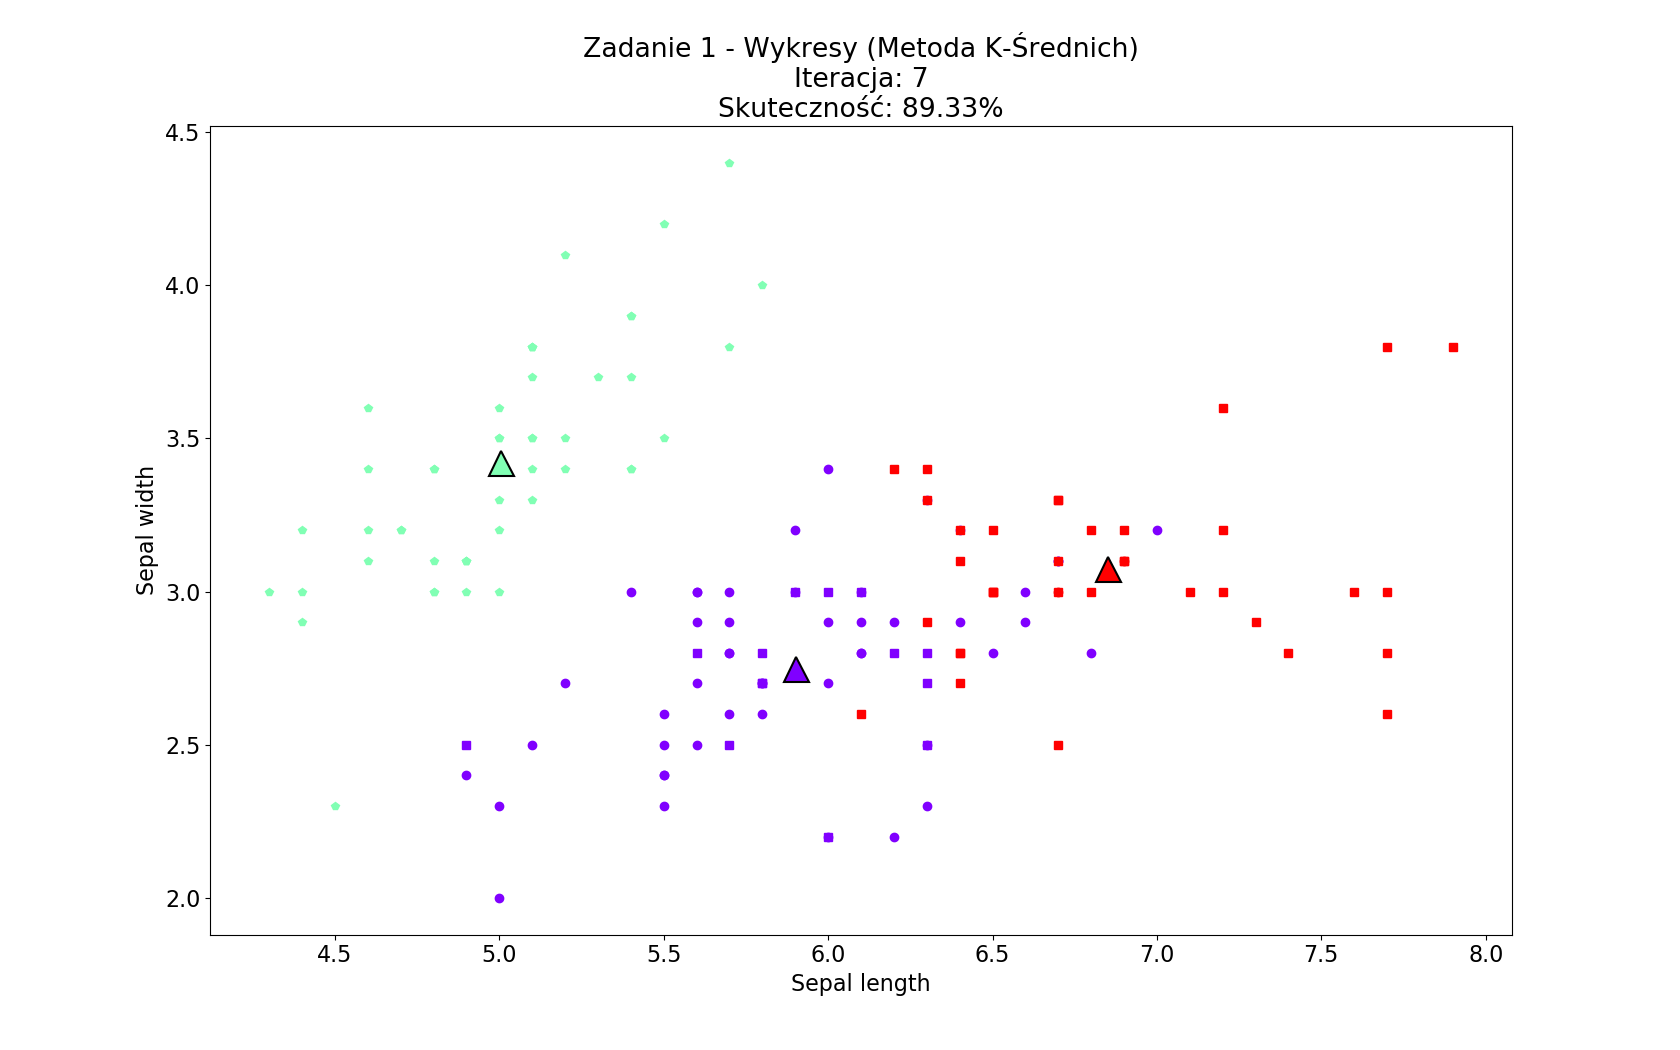
\includegraphics[width=\textwidth,width=105mm]{wykresy/plot_k_meansIrisDefault.png}
\caption{Tryb domyślny danych}
\end{figure}

\begin{figure}[!htbp]
\centering
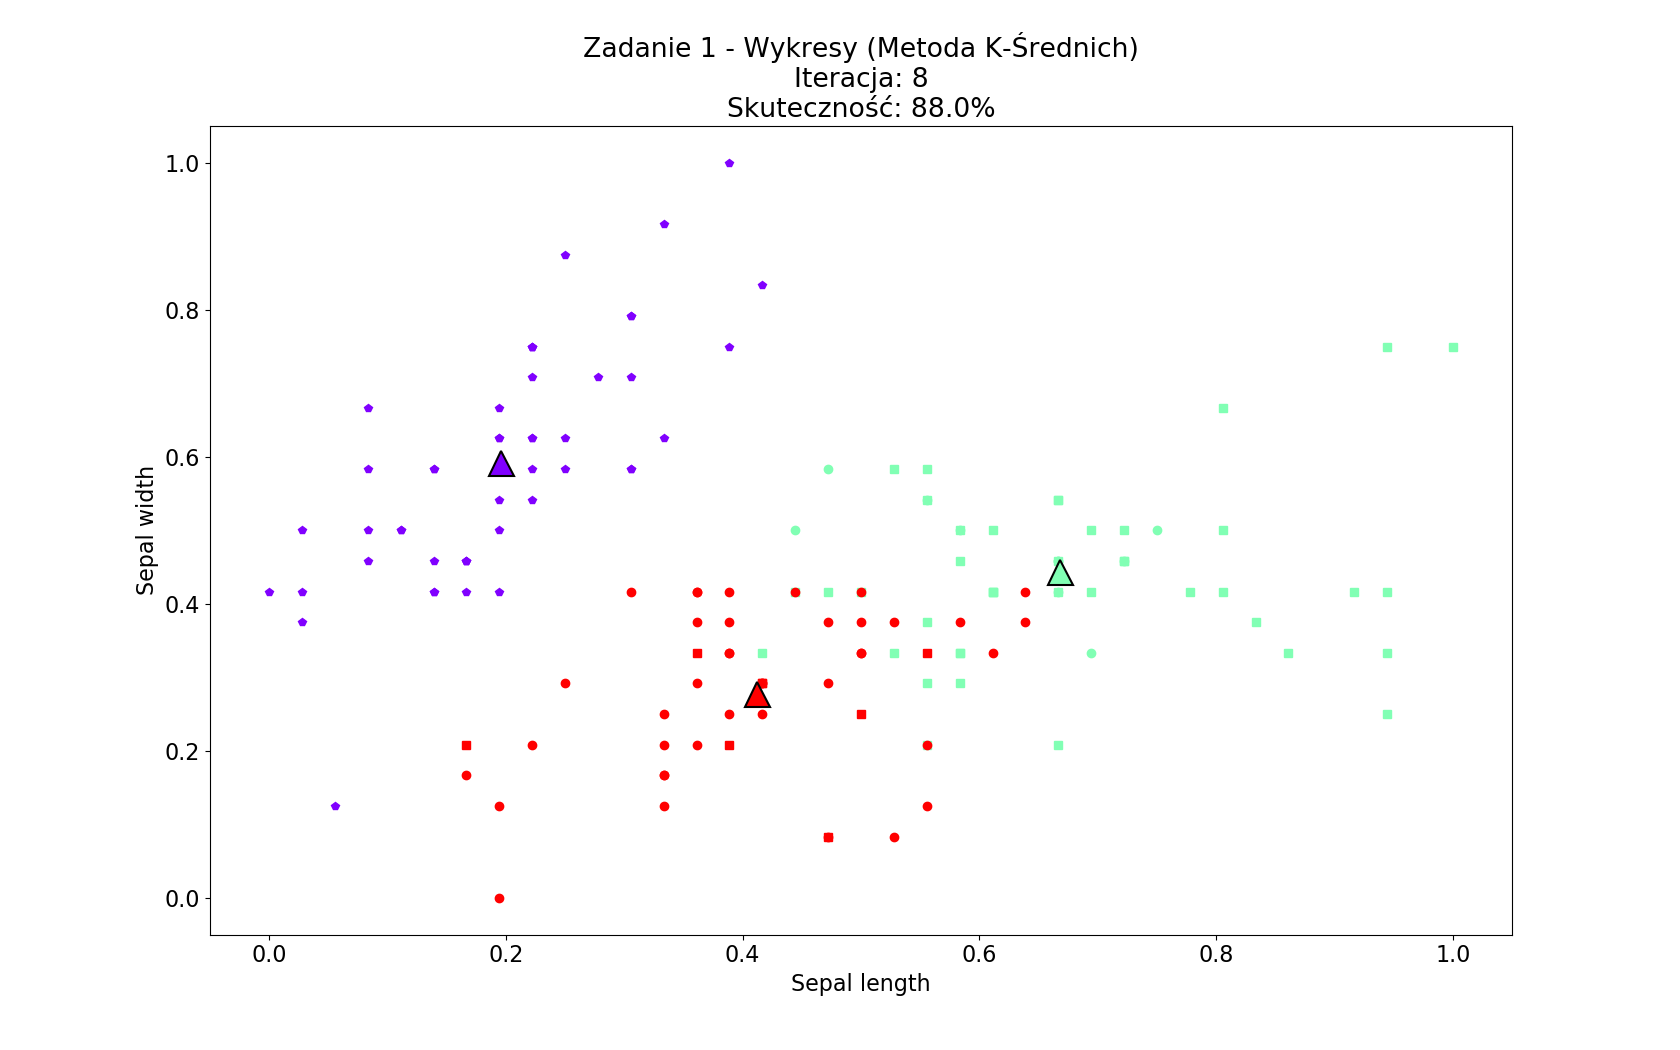
\includegraphics[width=\textwidth,width=105mm]{wykresy/plot_k_meansIrisNormalized.png}
\caption{Tryb normalizacji danych}
\end{figure}

\begin{figure}[!htbp]
\centering
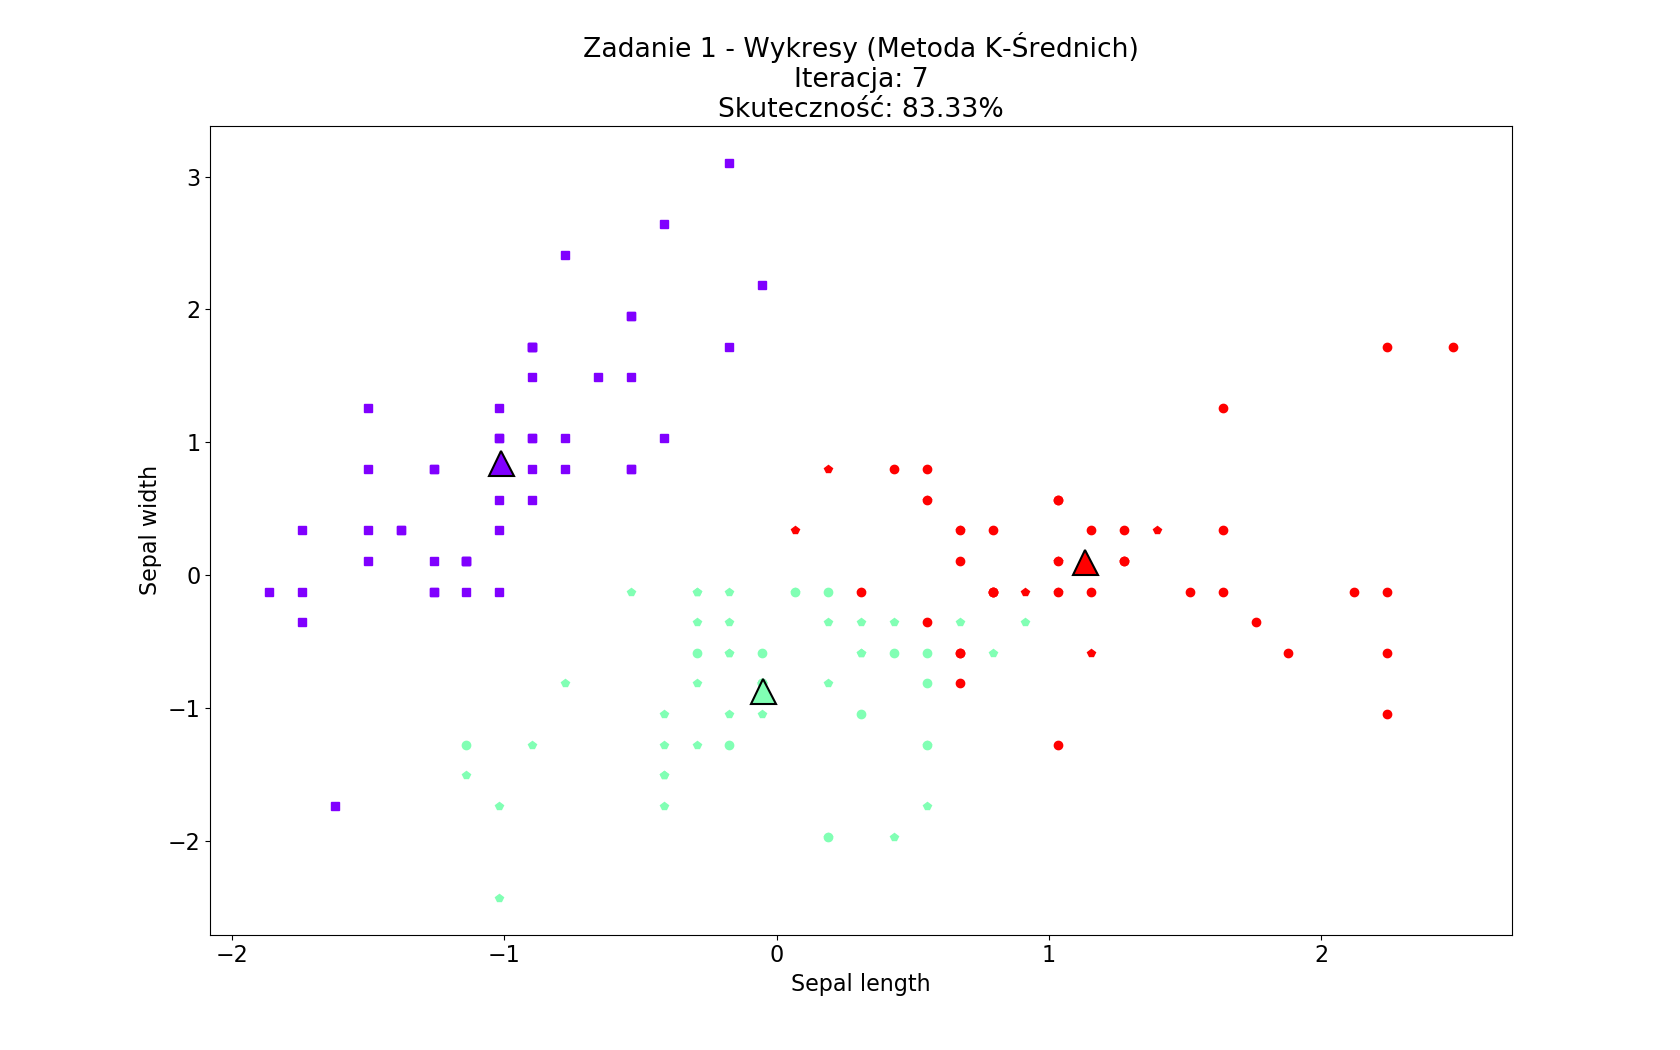
\includegraphics[width=\textwidth,width=105mm]{wykresy/plot_k_meansIrisStandadise.png}
\caption{Tryb standaryzacji danych}
\end{figure}
\FloatBarrier
}

\subsubsection{Algorytm Kohonena}
{
Poniżej wykresy dla trzech trybów
\begin{figure}[!htbp]
\centering
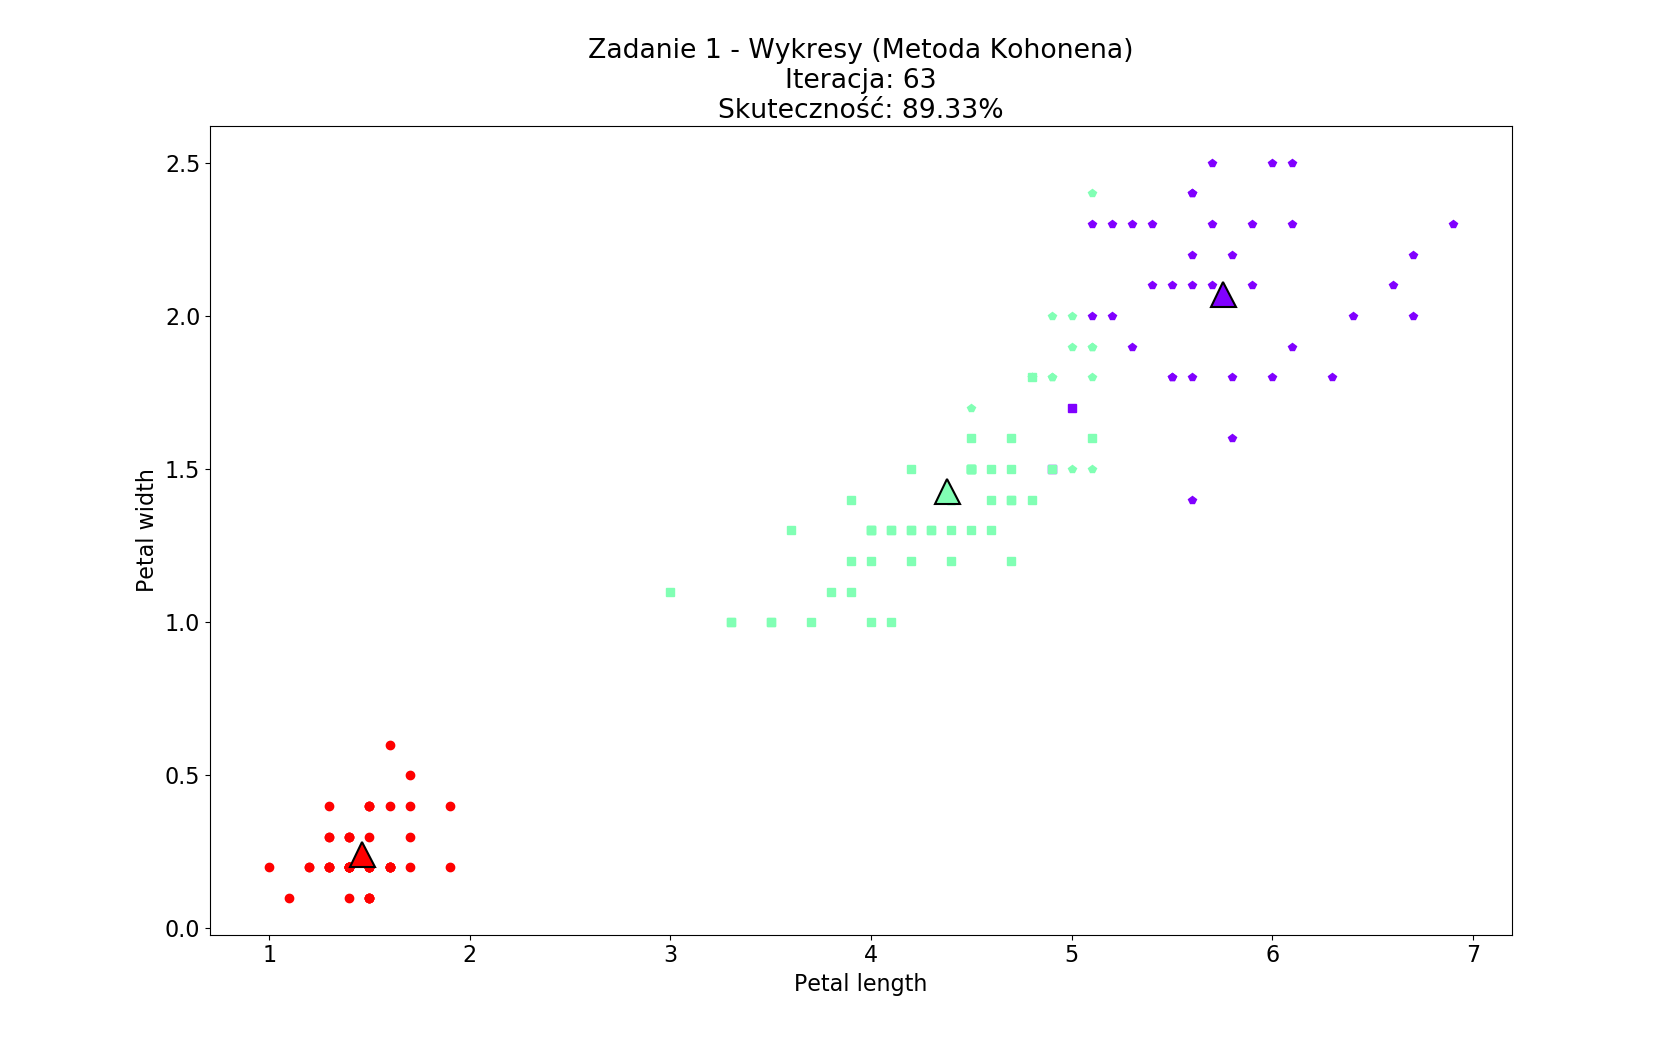
\includegraphics[width=\textwidth,width=95mm]{wykresy/plot_kohonenIrisDefault.png}
\caption{Tryb domyślny danych}
\end{figure}

\begin{figure}[!htbp]
\centering
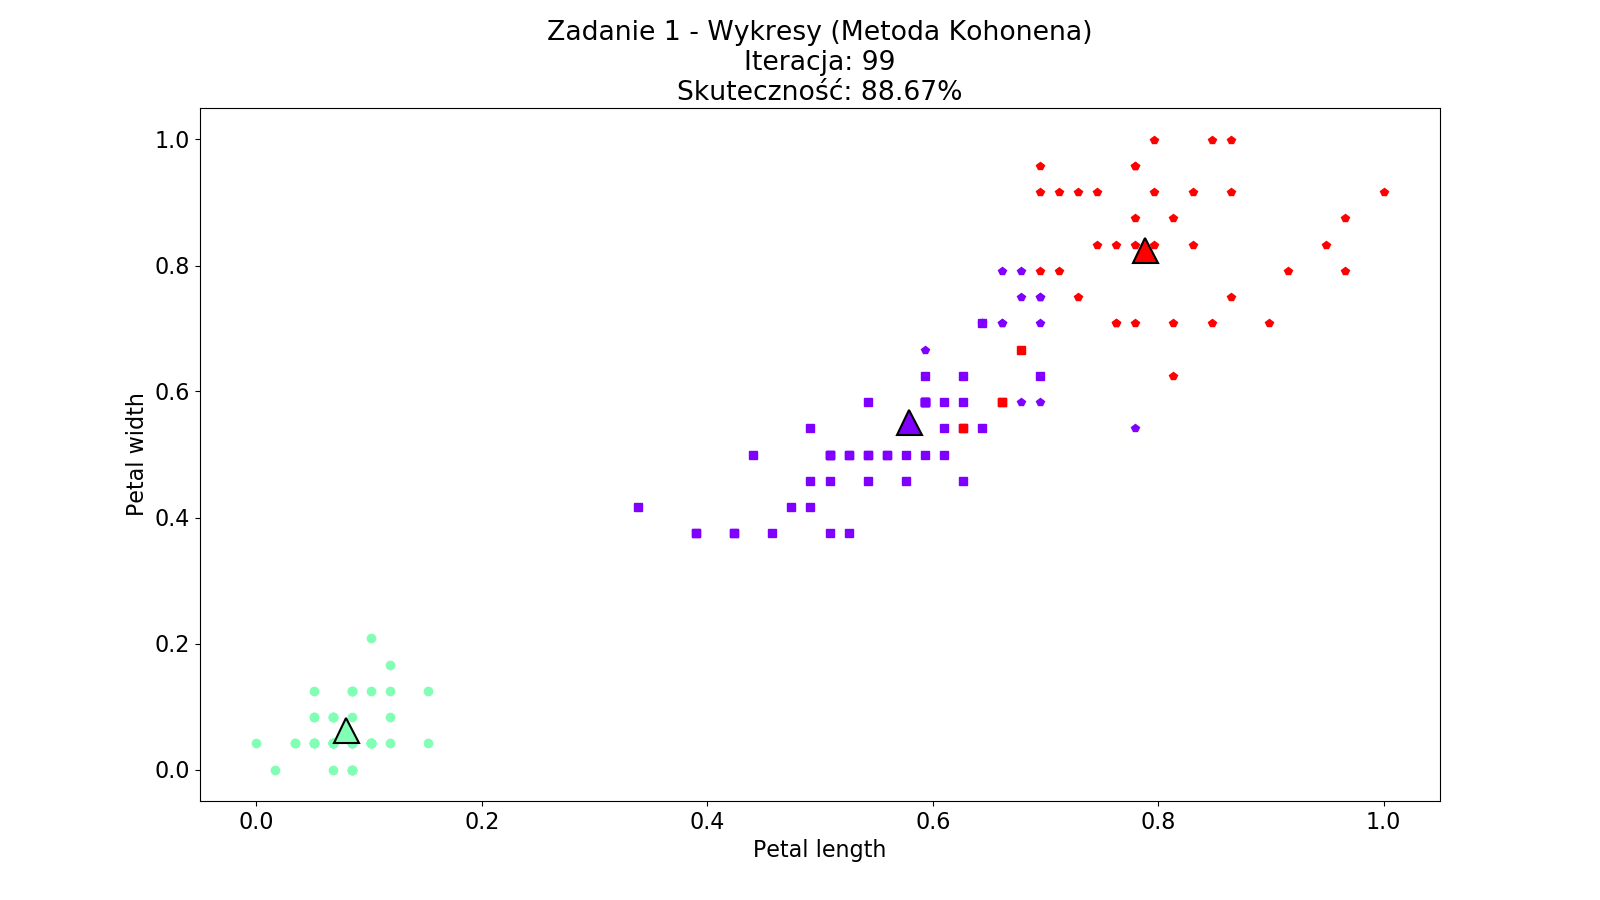
\includegraphics[width=\textwidth,width=95mm]{wykresy/plot_kohonenIrisNormalized.png}
\caption{Tryb normalizacji danych}
\end{figure}

\begin{figure}[!htbp]
\centering
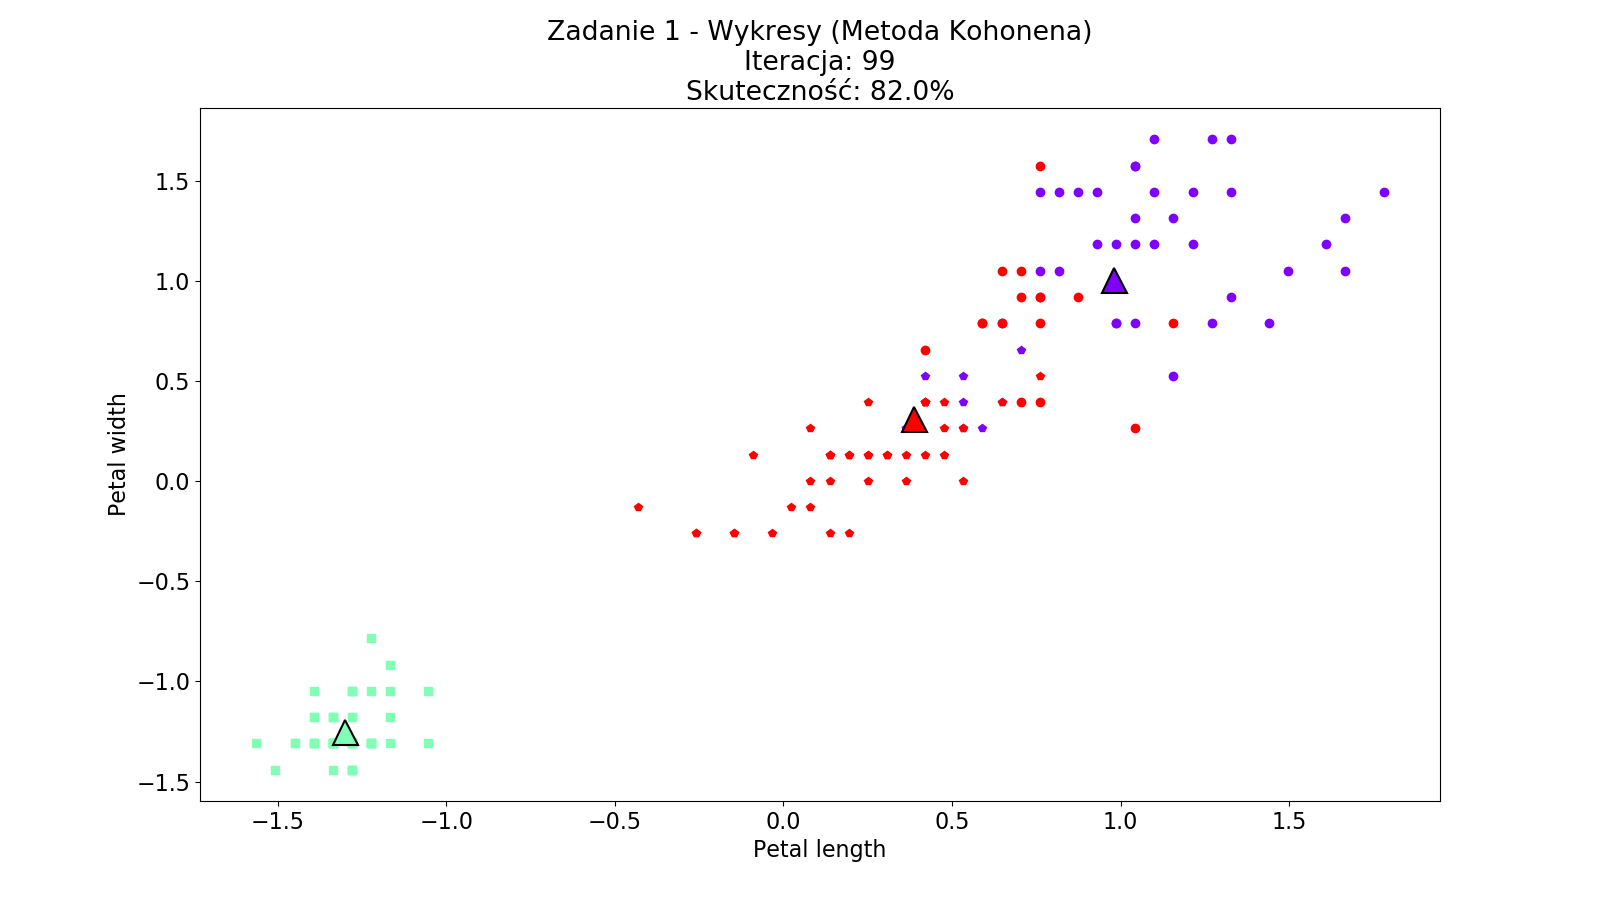
\includegraphics[width=\textwidth,width=95mm]{wykresy/plot_kohonenIrisStandardised.png}
\caption{Tryb standaryzacji danych}
\end{figure}
\FloatBarrier
}

}
\subsection{Zbiór win}
{
\subsubsection{Algorytm k - średnich}
{
Poniżej wykresy dla trzech trybów
\begin{figure}[!htbp]
\centering
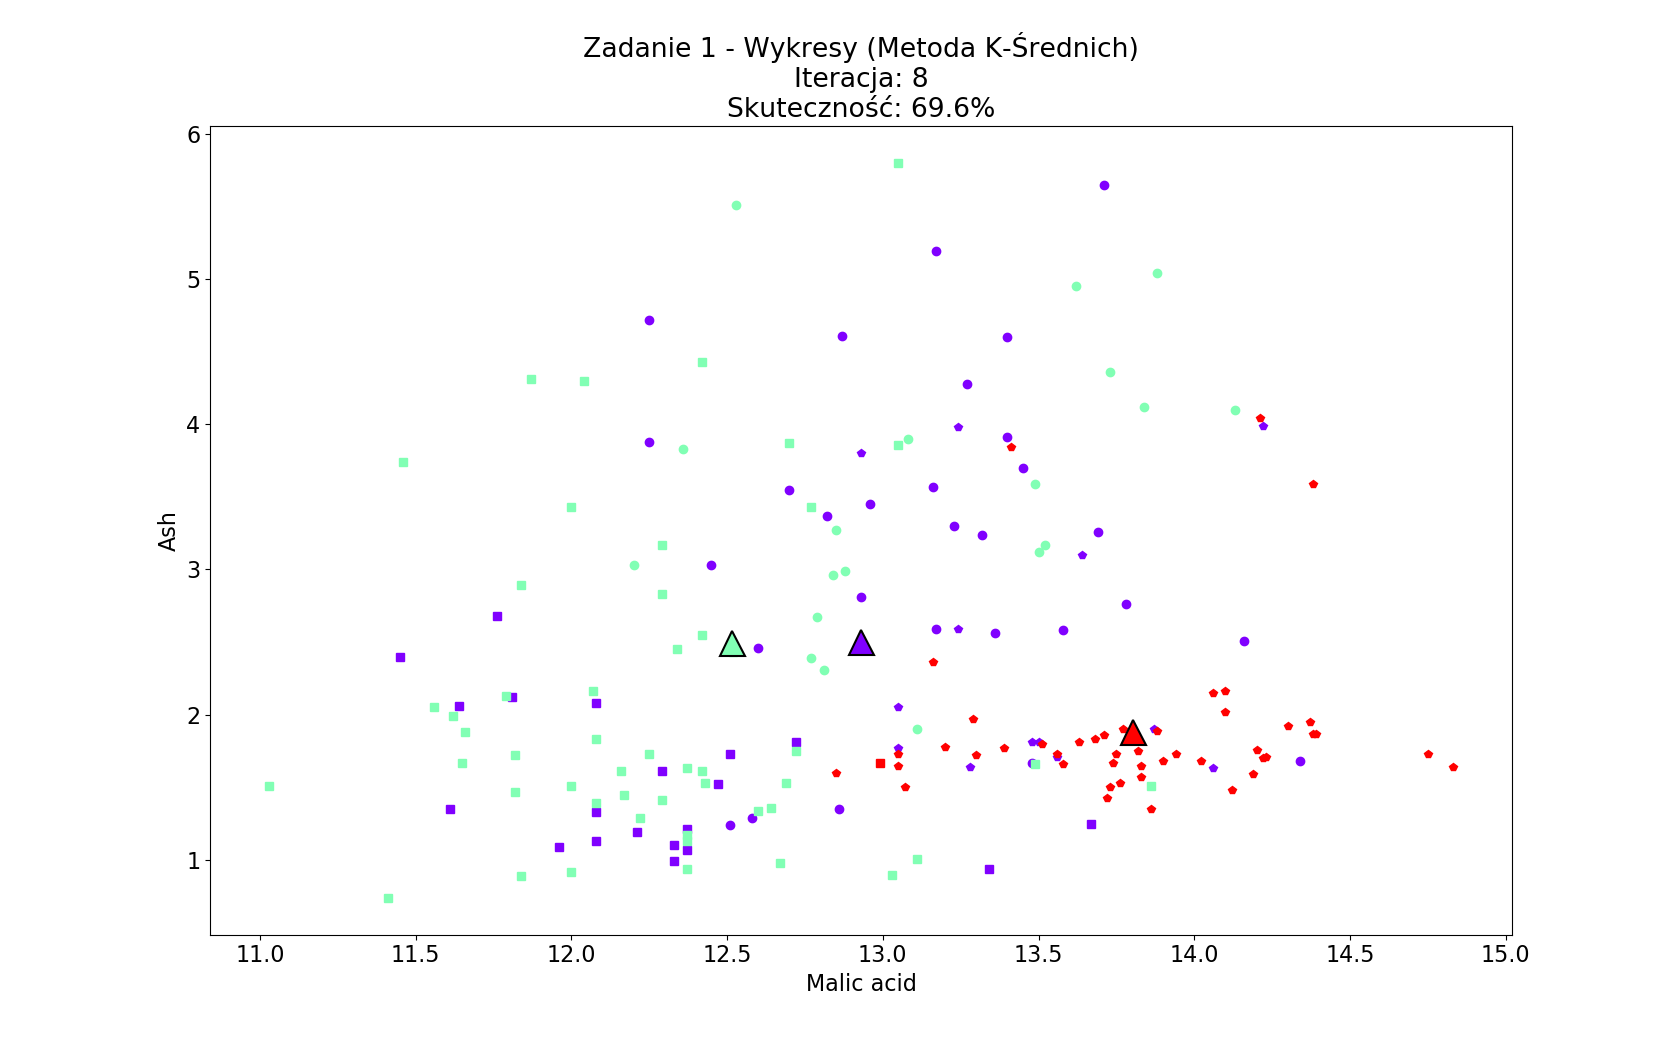
\includegraphics[width=\textwidth,width=85mm]{wykresy/plot_k_meansWineDefault.png}
\caption{Tryb domyślny danych}
\end{figure}

\begin{figure}[!htbp]
\centering
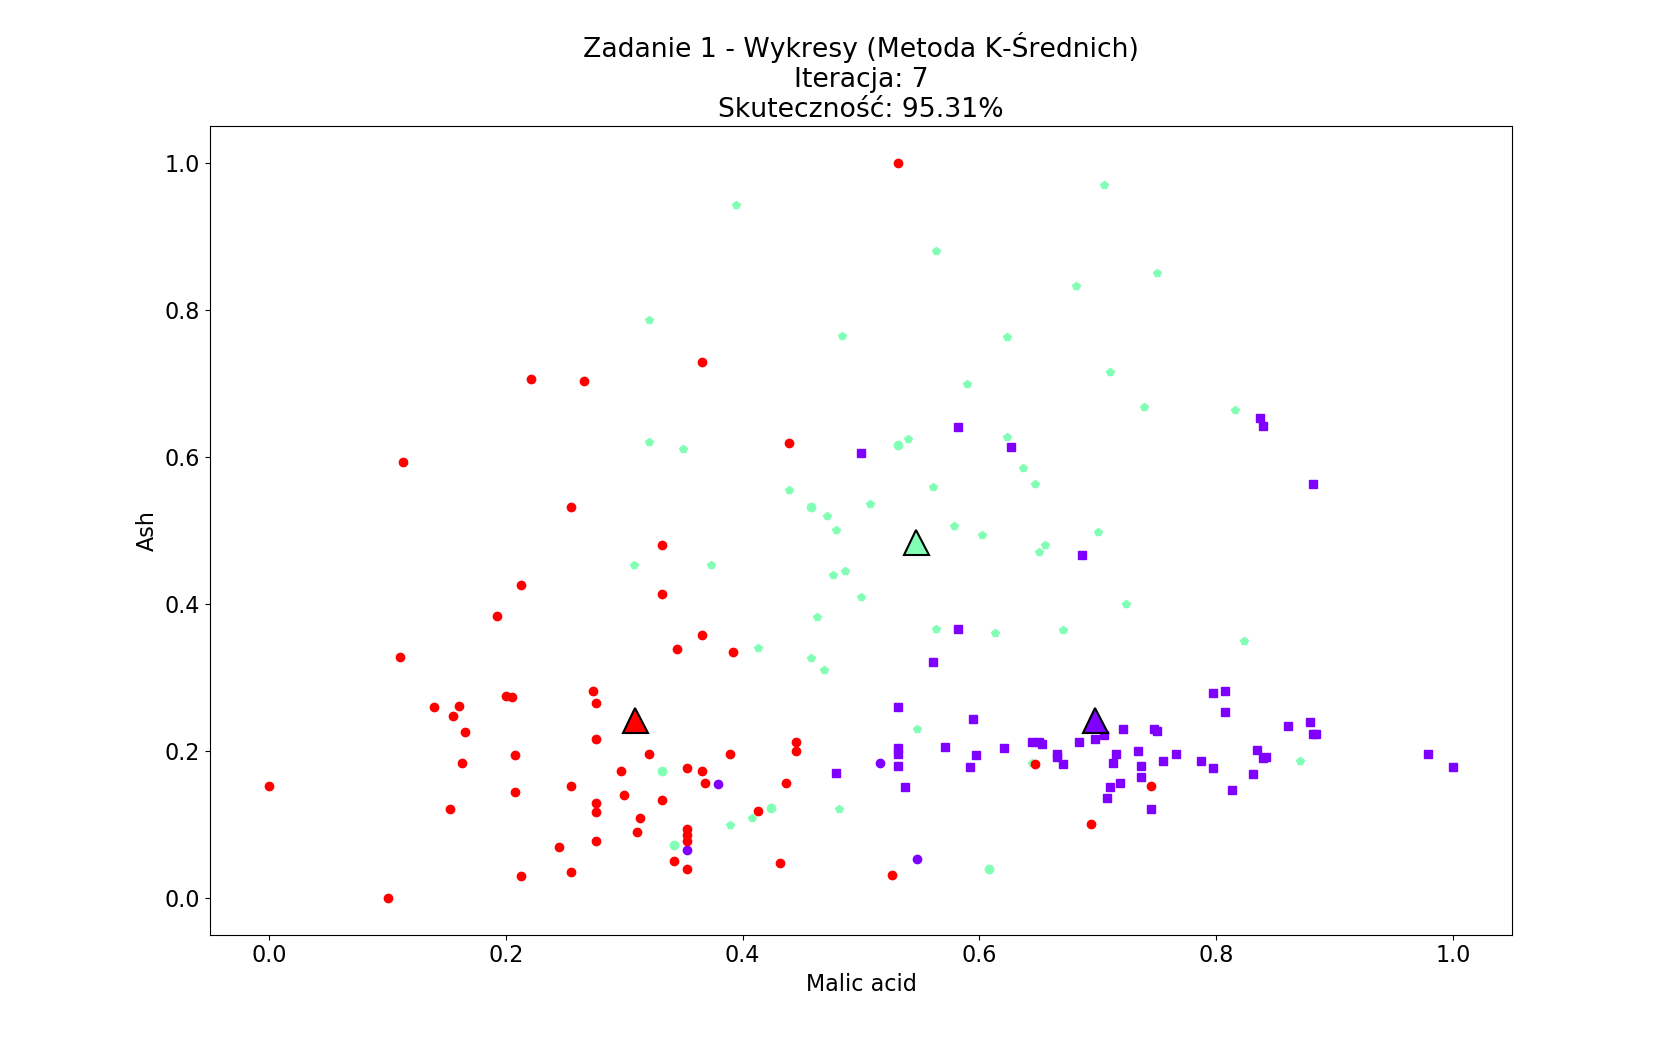
\includegraphics[width=\textwidth,width=85mm]{wykresy/plot_k_meansWineNormalised.png}
\caption{Tryb normalizacji danych}
\end{figure}

\begin{figure}[!htbp]
\centering
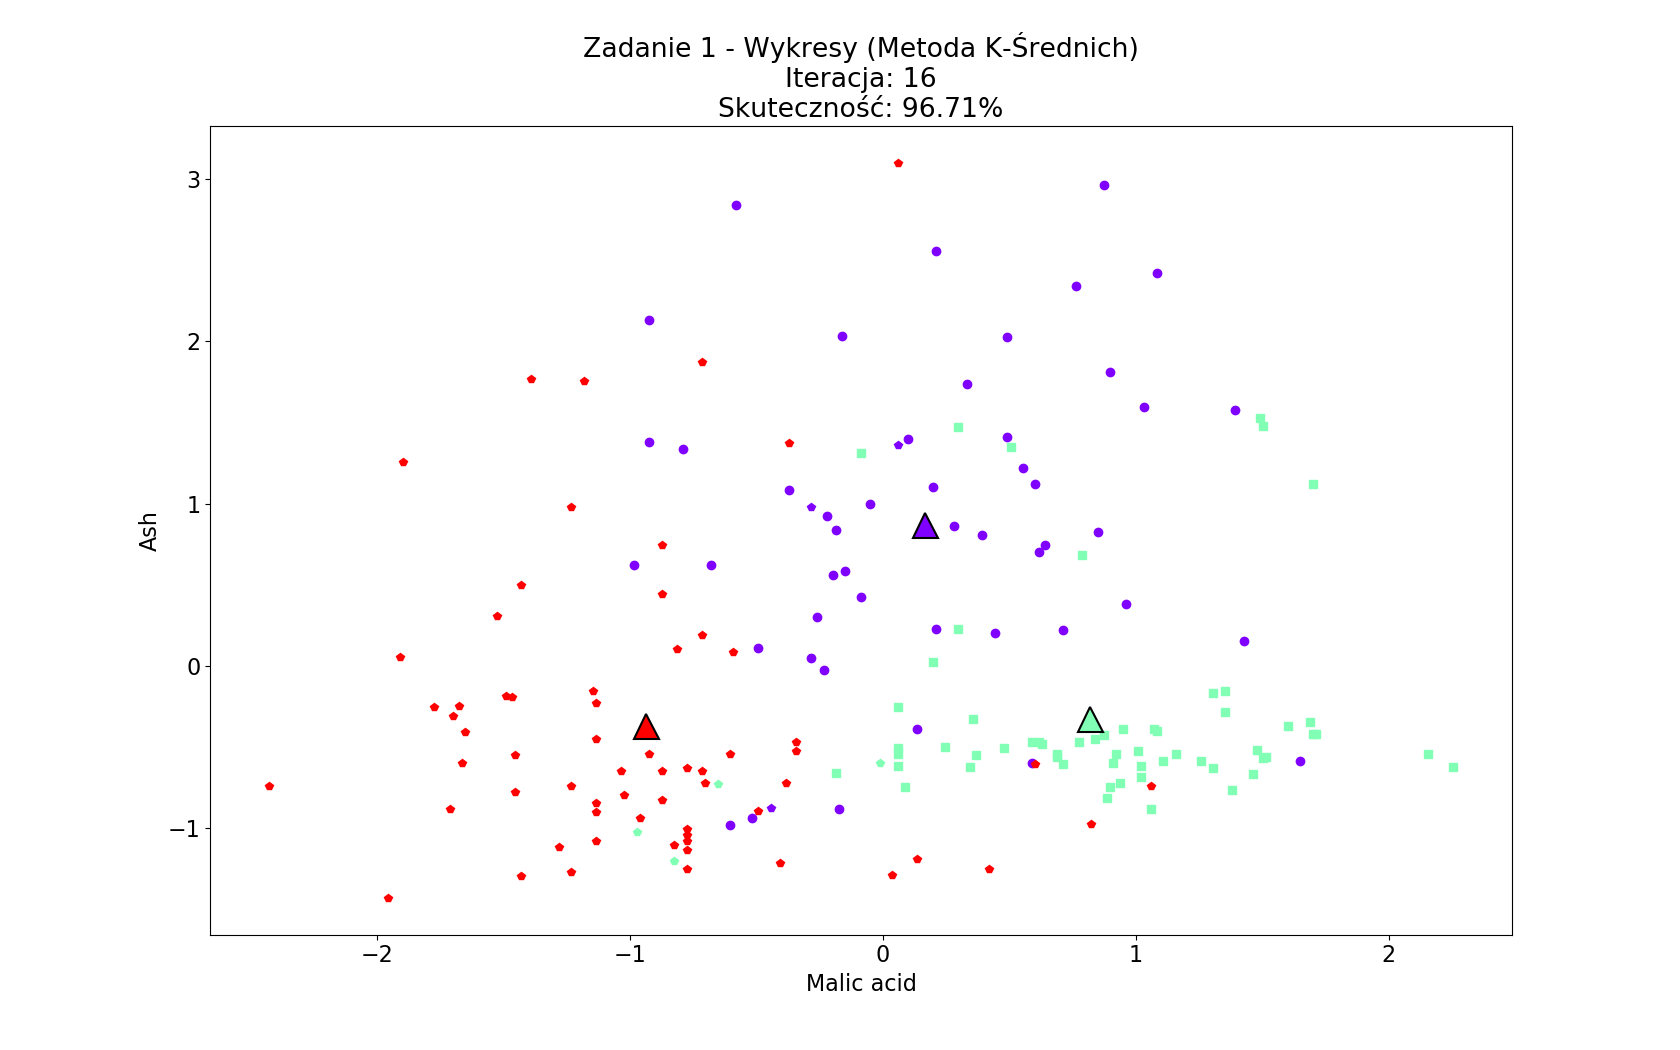
\includegraphics[width=\textwidth,width=85mm]{wykresy/plot_k_meansWineStandardise.png}
\caption{Tryb standaryzacji danych}
\end{figure}
\FloatBarrier
}

\subsubsection{Algorytm Kohonena}
{
Poniżej wykresy dla trzech trybów
\begin{figure}[!htbp]
\centering
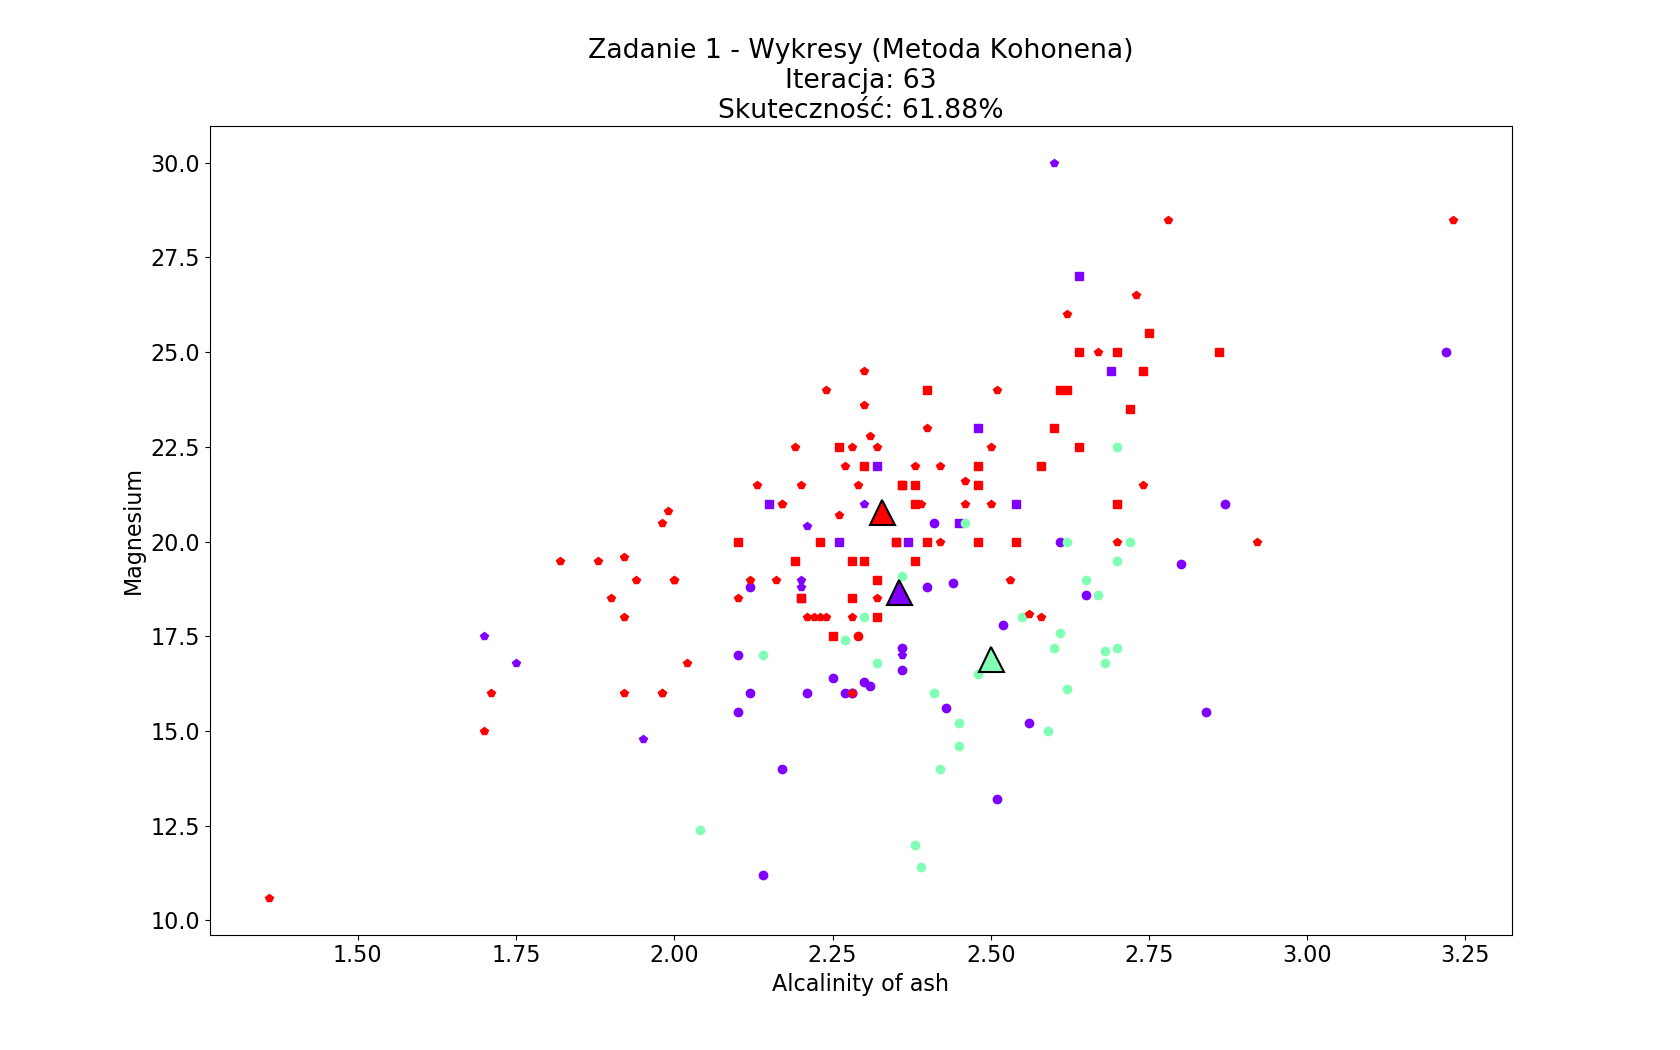
\includegraphics[width=\textwidth,width=85mm]{wykresy/plot_kohonenWineDefault.png}
\caption{Tryb domyślny danych}
\end{figure}

\begin{figure}[!htbp]
\centering
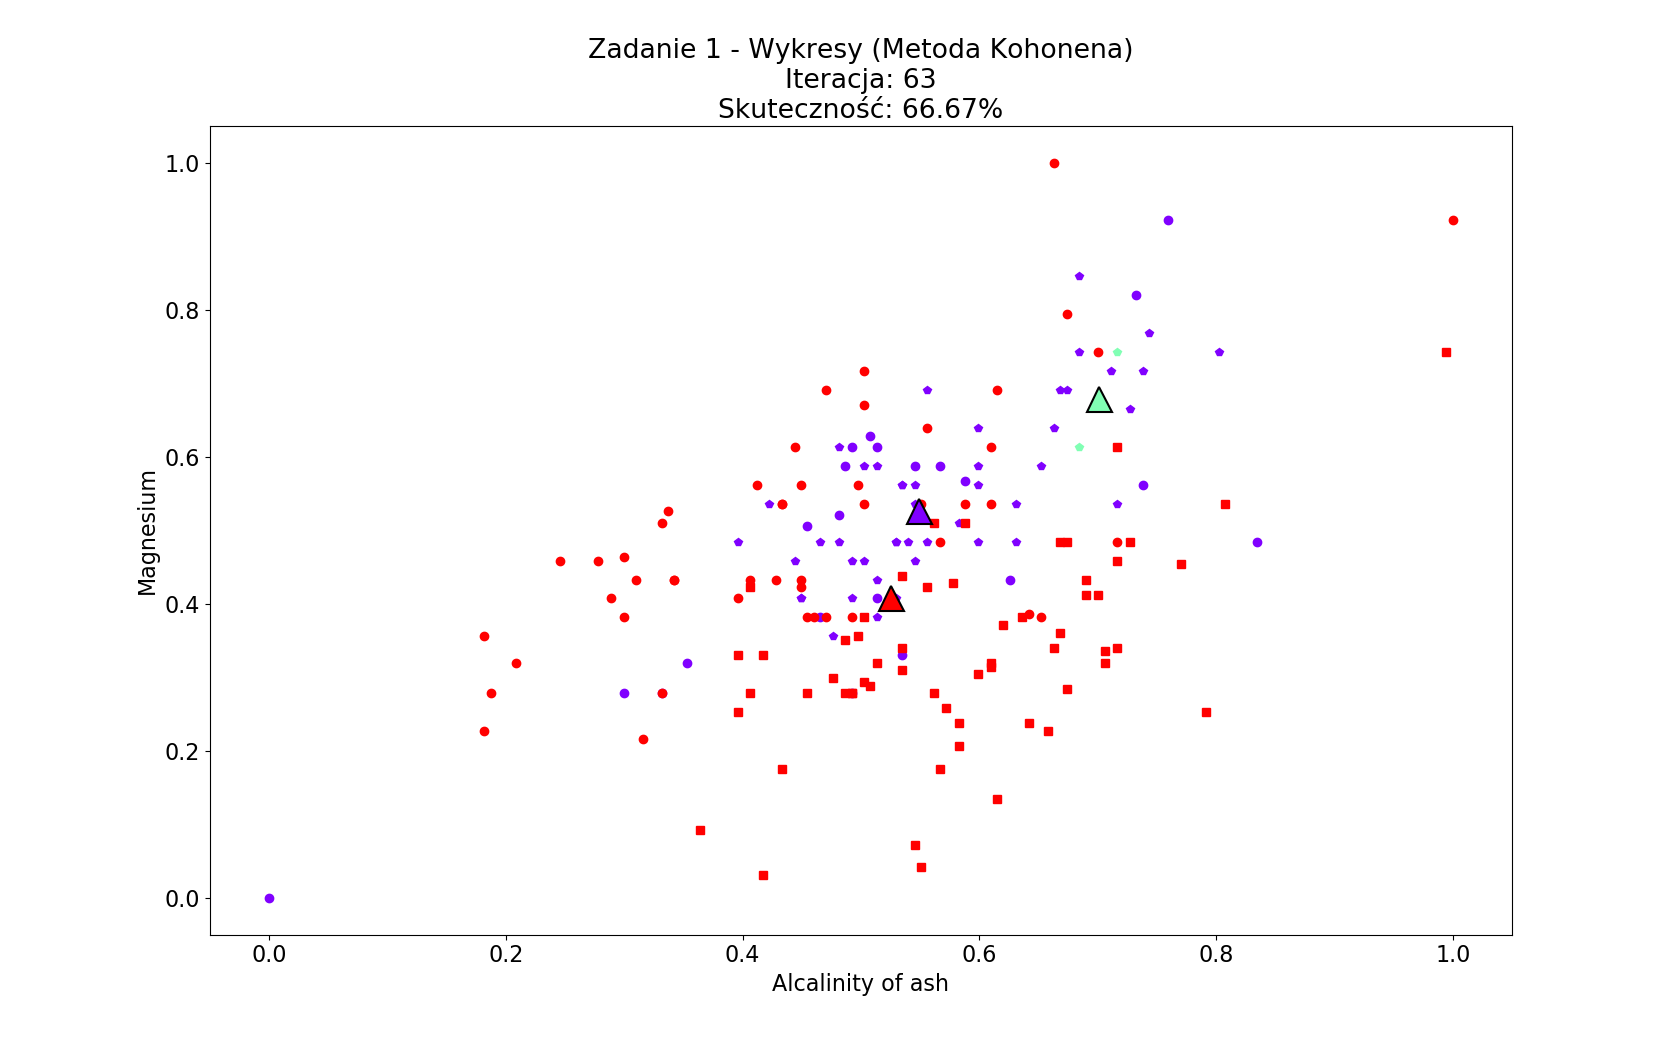
\includegraphics[width=\textwidth,width=85mm]{wykresy/plot_kohonenWineNormalised.png}
\caption{Tryb normalizacji danych}
\end{figure}

\begin{figure}[!htbp]
\centering
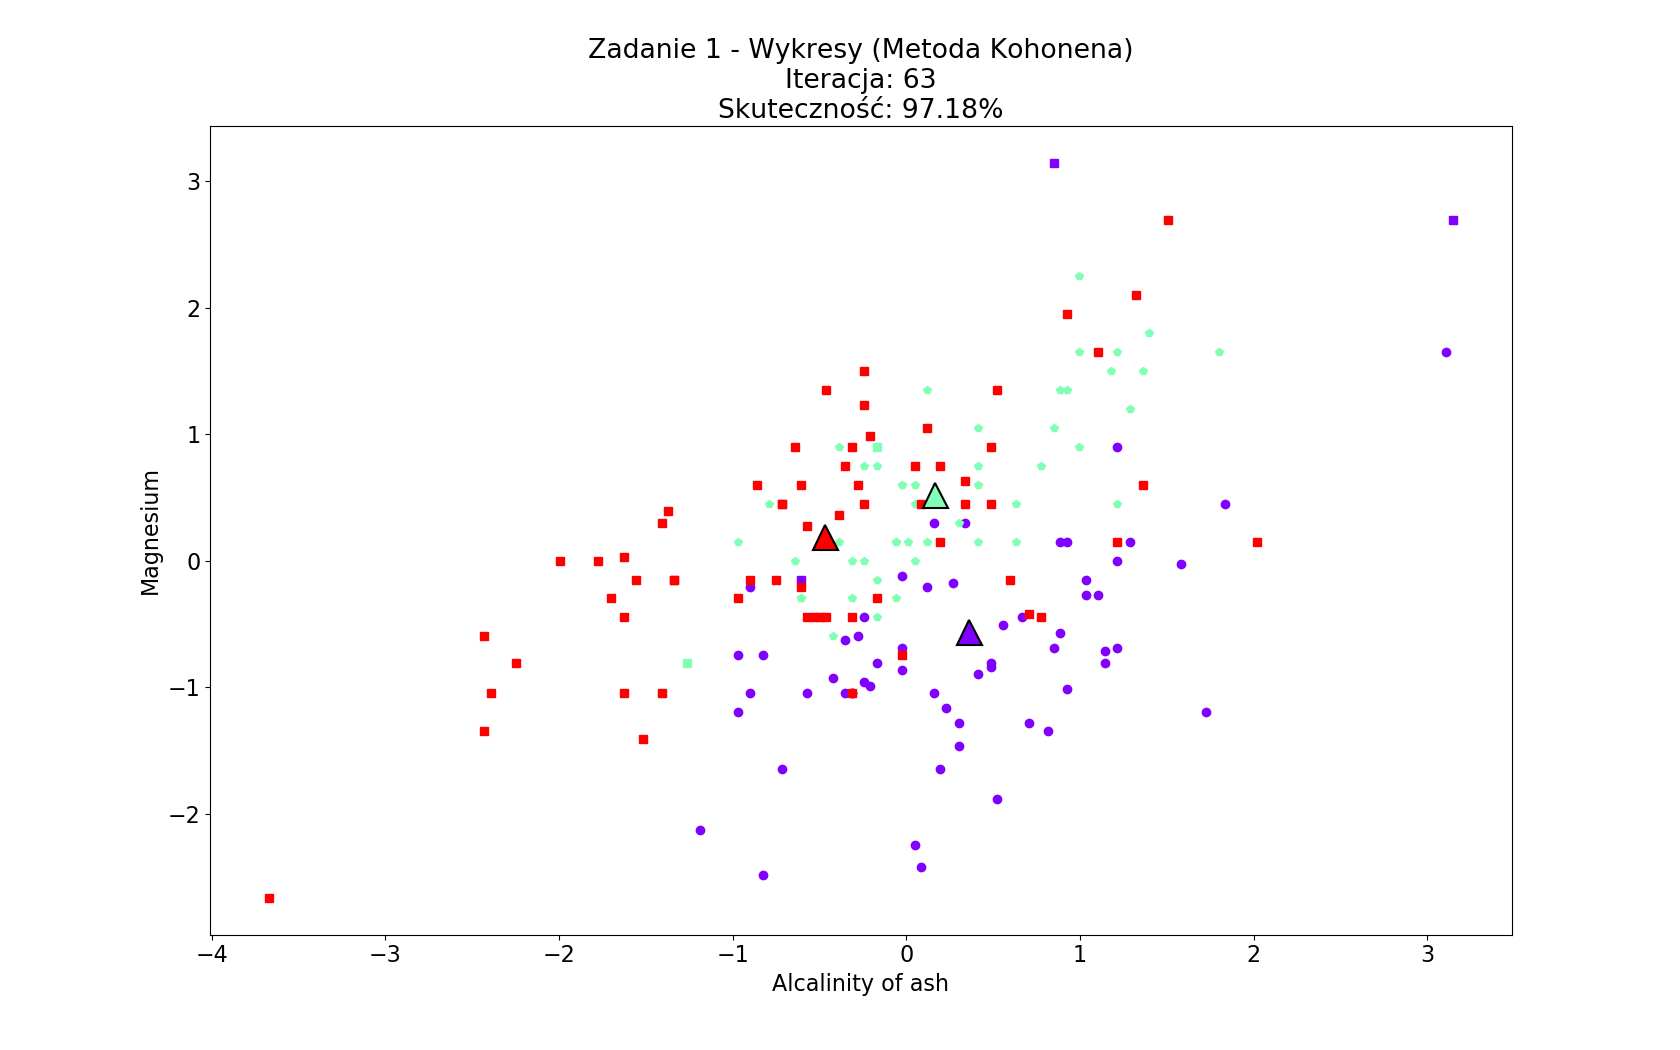
\includegraphics[width=\textwidth,width=85mm]{wykresy/plot_kohonenWineStandardised.png}
\caption{Tryb standaryzacji danych}
\end{figure}
\FloatBarrier
}

}
\subsection{Zbiór abalone}
{
\subsubsection{Algorytm k - średnich}
{
Poniżej wykresy dla trzech trybów
\begin{figure}[!htbp]
\centering
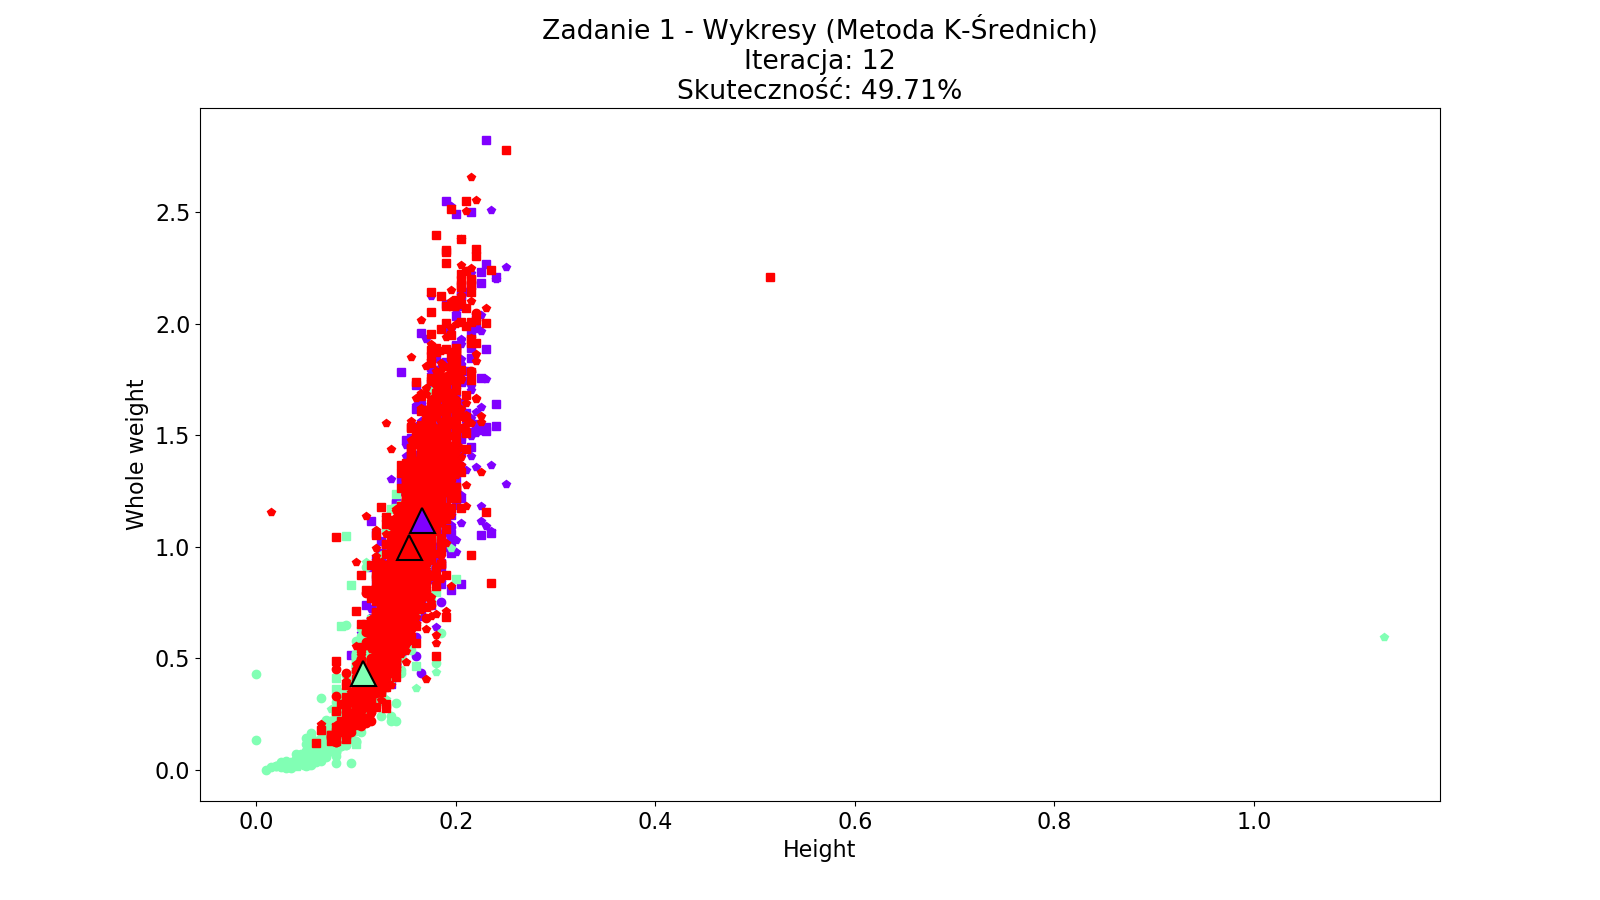
\includegraphics[width=\textwidth,width=95mm]{wykresy/plot_k_meansAbaloneDefault.png}
\caption{Tryb domyślny danych}
\end{figure}

\begin{figure}[!htbp]
\centering
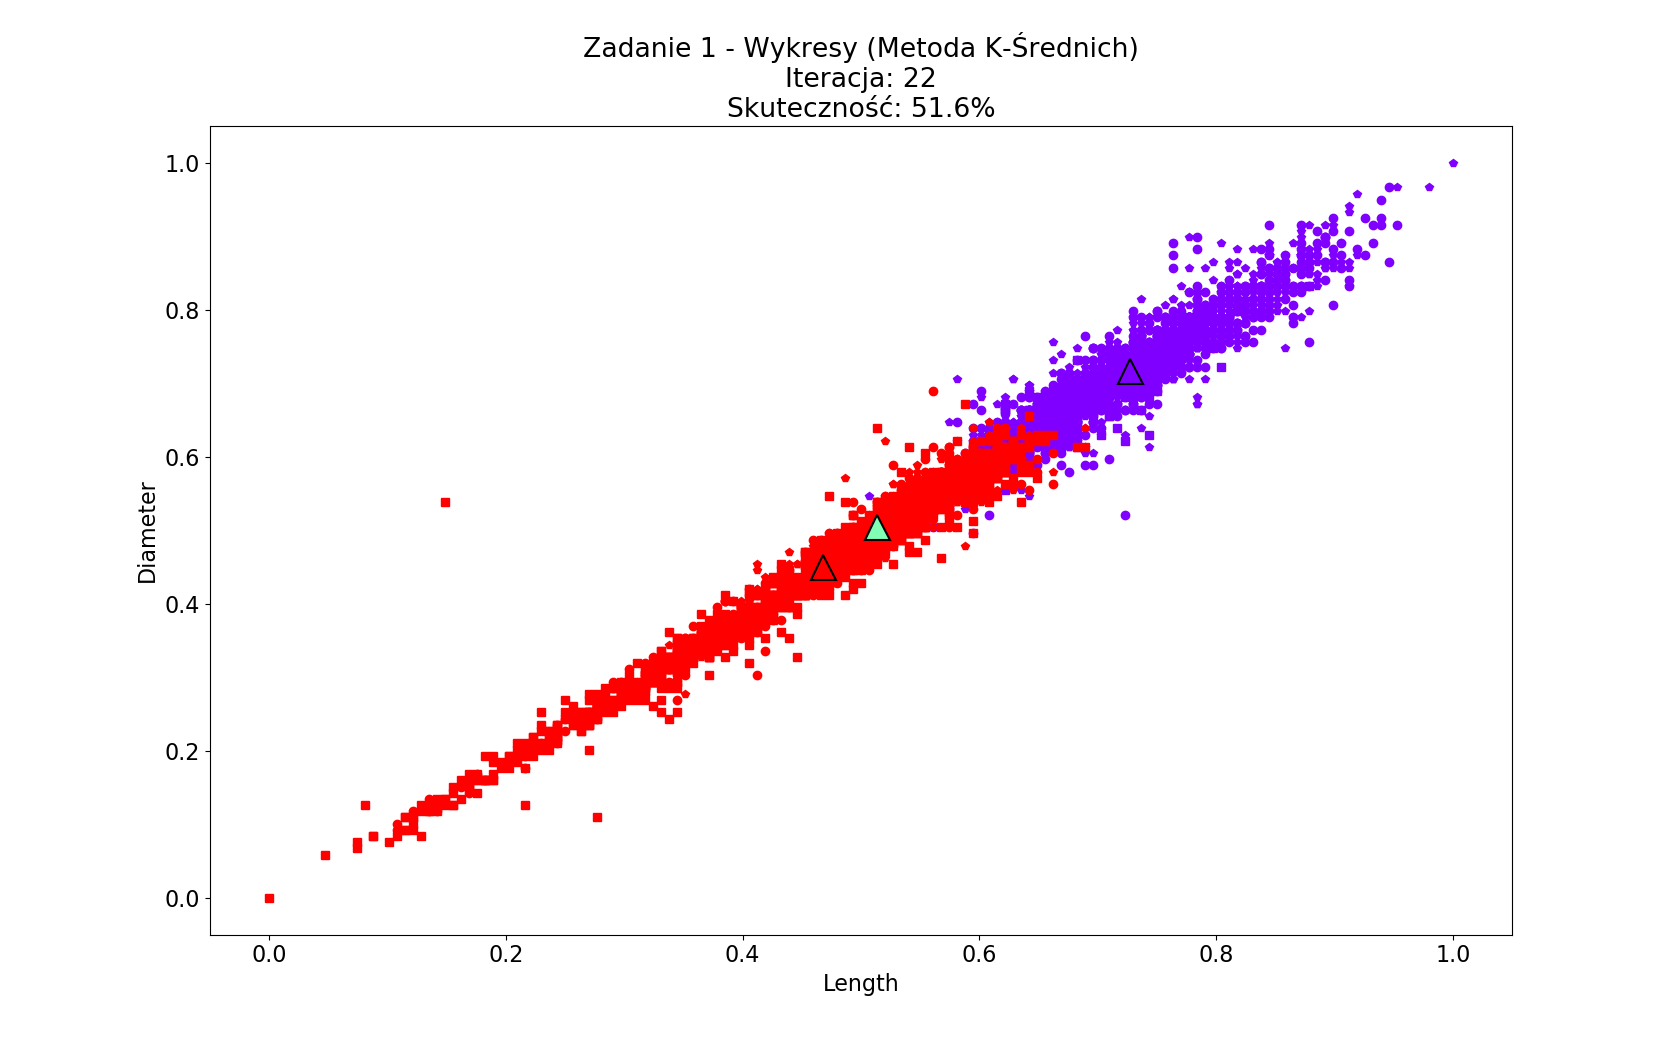
\includegraphics[width=\textwidth,width=95mm]{wykresy/plot_k_meansAbaloneNormalised.png}
\caption{Tryb normalizacji danych}
\end{figure}

\begin{figure}[!htbp]
\centering
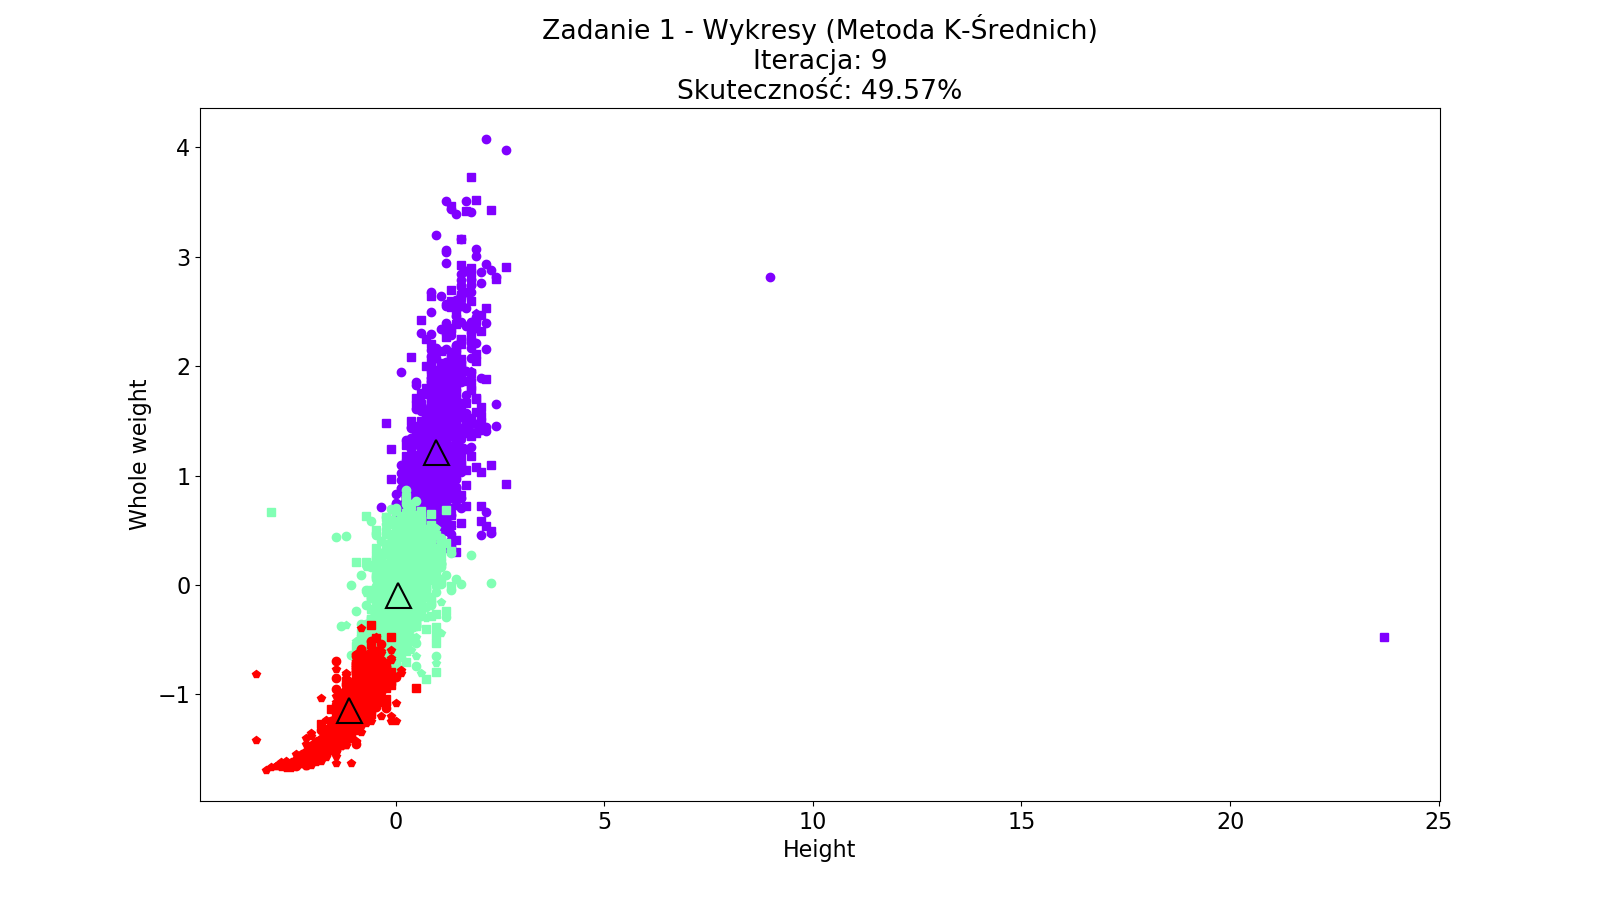
\includegraphics[width=\textwidth,width=95mm]{wykresy/plot_k_meansAbaloneStandardise.png}
\caption{Tryb standaryzacji danych}
\end{figure}
\FloatBarrier
}

\subsubsection{Algorytm Kohonena}
{
Poniżej wykresy dla trzech trybów
\begin{figure}[!htbp]
\centering
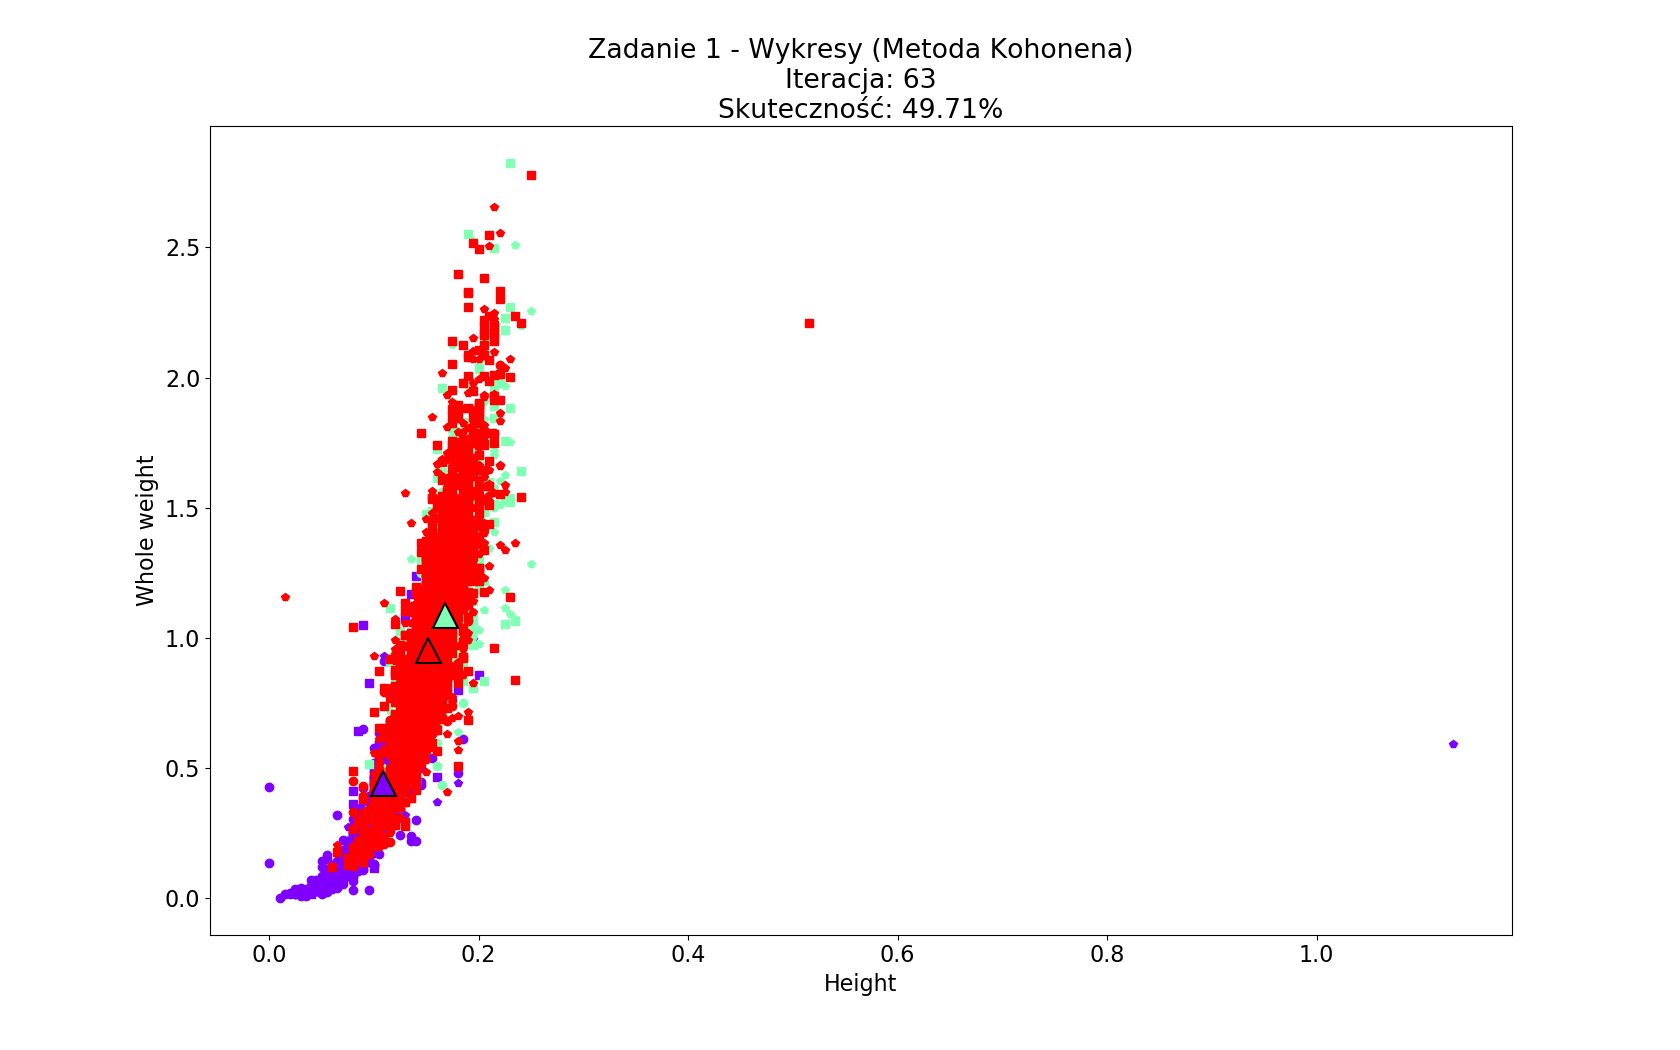
\includegraphics[width=\textwidth,width=90mm]{wykresy/plot_kohonenAbaloneDefault.png}
\caption{Tryb domyślny danych}
\end{figure}

\begin{figure}[!htbp]
\centering
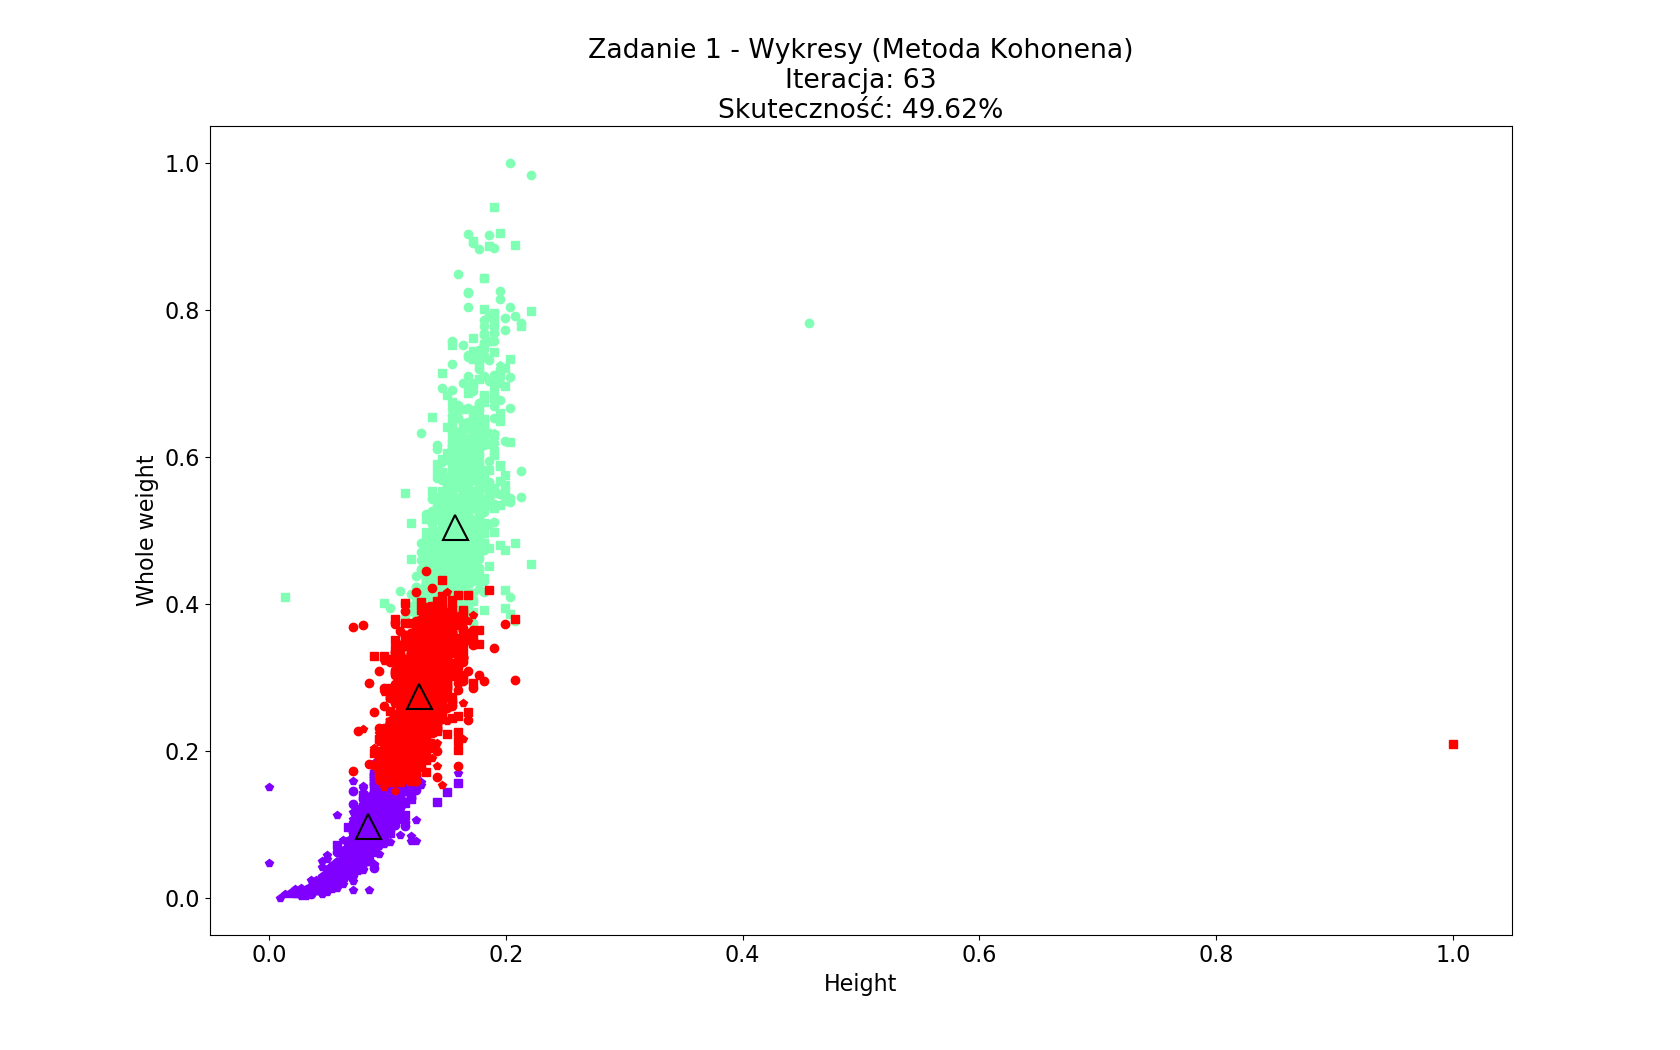
\includegraphics[width=\textwidth,width=90mm]{wykresy/plot_kohonenAbaloneNormalised.png}
\caption{Tryb normalizacji danych}
\end{figure}

\begin{figure}[!htbp]
\centering
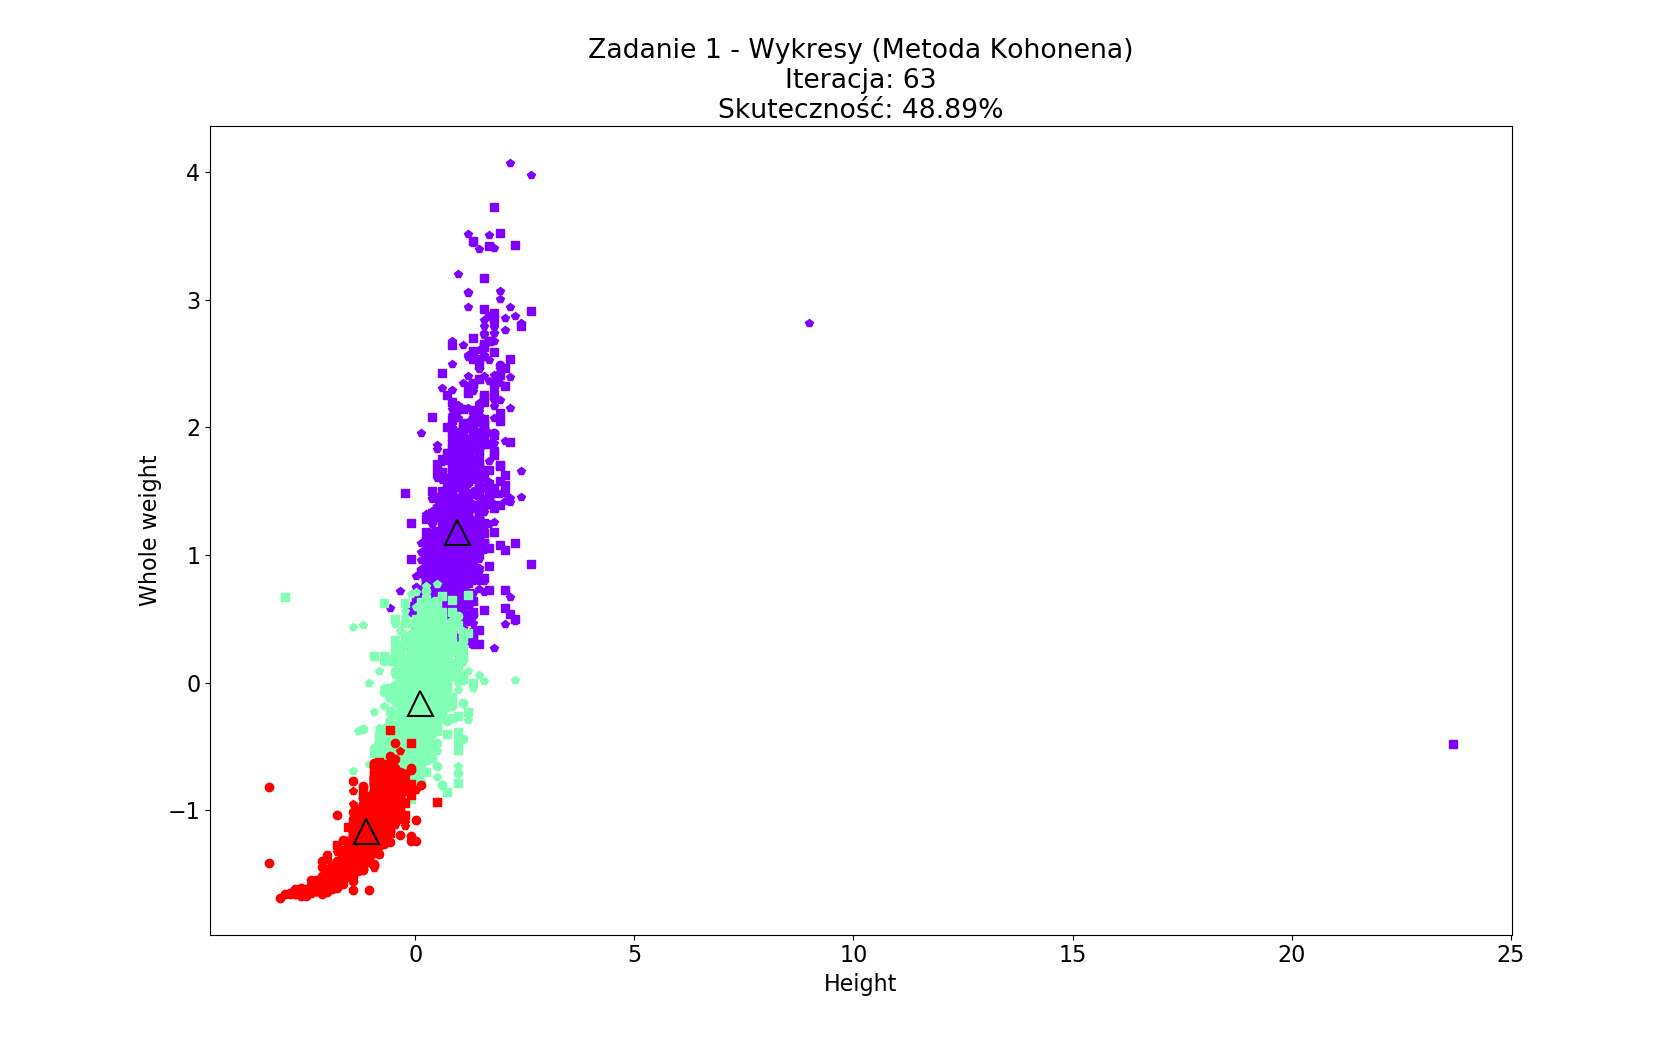
\includegraphics[width=\textwidth,width=90mm]{wykresy/plot_kohonenAbaloneStandardised.png}
\caption{Tryb standaryzacji danych}
\end{figure}
\FloatBarrier
}

\subsection{Obrazy Algorytm k - średnich}
{
\subsubsection{chair.png}
{

Poniżej obrazy dla róznych rozmiarów ramek
\begin{figure}[!htbp]
\centering
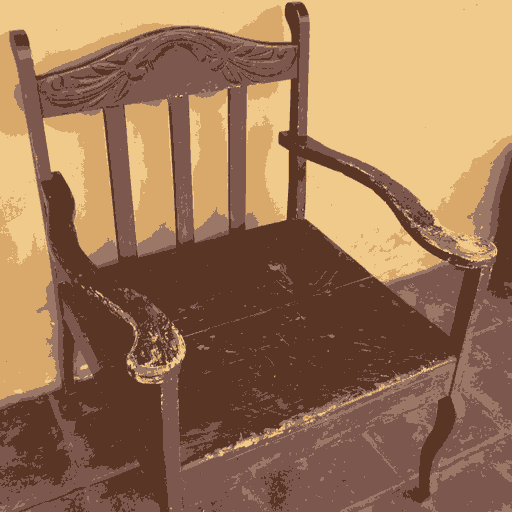
\includegraphics[width=\textwidth,width=90mm]{obrazy/chair_R1_K5_P1_It10.png}
\caption{Rozmiar ramek: 1 liczba klastrów: 5 powtórzenia: 1 iteracje: 10 }
\end{figure}

\begin{figure}[!htbp]
\centering
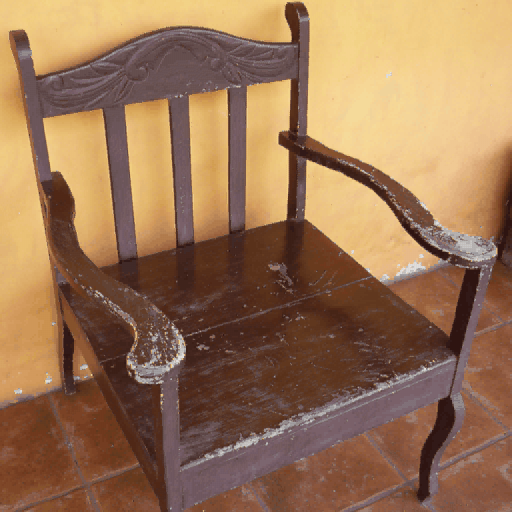
\includegraphics[width=\textwidth,width=90mm]{obrazy/chair_R2_K256_P1_It10.png}
\caption{Rozmiar ramek: 2 liczba klastrów:256 powtórzenia: 1 iteracje: 10 }
\end{figure}

\begin{figure}[!htbp]
\centering
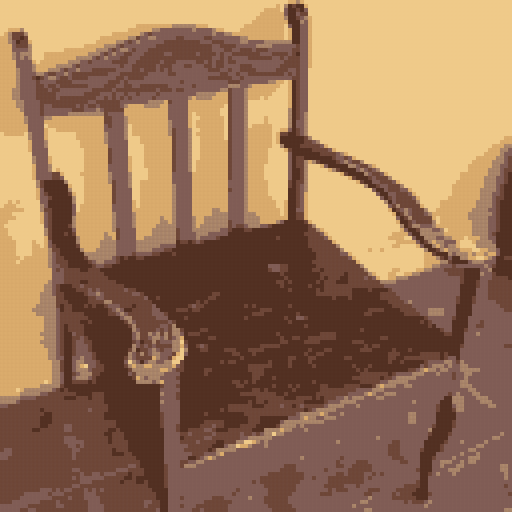
\includegraphics[width=\textwidth,width=90mm]{obrazy/chair_R4_K6_P1_It10.png}
\caption{Rozmiar ramek: 4 liczba klastrów:6 powtórzenia: 1 iteracje: 10 }
\end{figure}

\begin{figure}[!htbp]
\centering
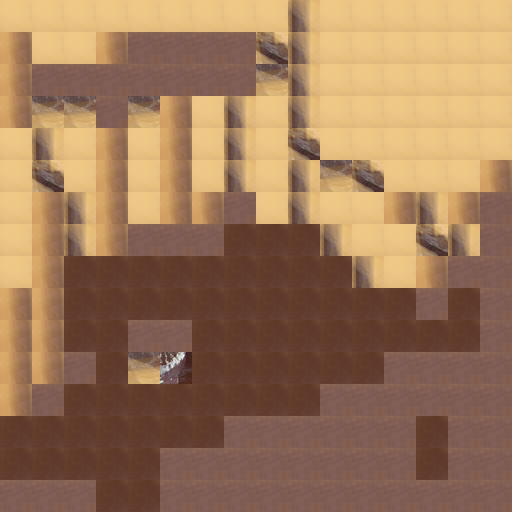
\includegraphics[width=\textwidth,width=90mm]{obrazy/chair_R32_K8_P1_It10.png}
\caption{Rozmiar ramek: 32 liczba klastrów:8 powtórzenia: 1 iteracje: 10 }
\end{figure}

\begin{figure}[!htbp]
\centering
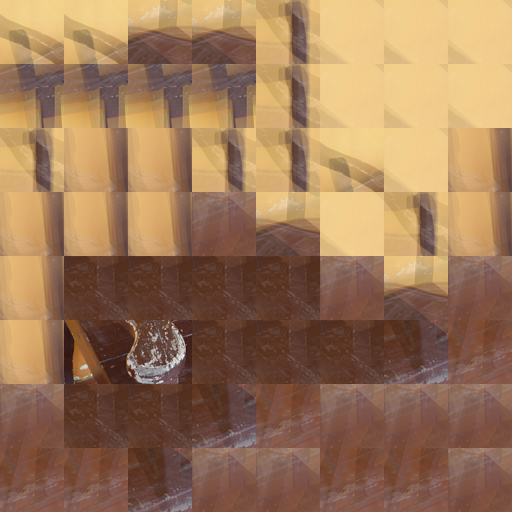
\includegraphics[width=\textwidth,width=90mm]{obrazy/chair_R64_K12_P1_It10.png}
\caption{Rozmiar ramek: 64 liczba klastrów:12 powtórzenia: 1 iteracje: 10 }
\end{figure}
\FloatBarrier
}

\subsubsection{house.png}
{

Poniżej obrazy dla róznych rozmiarów ramek
\begin{figure}[!htbp]
\centering
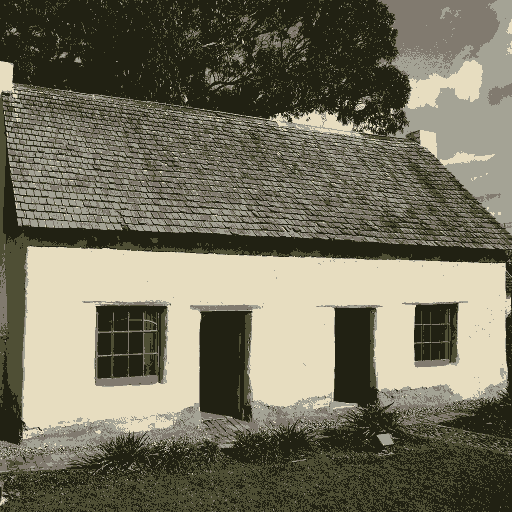
\includegraphics[width=\textwidth,width=90mm]{obrazy/house_R1_K5_P1_It10.png}
\caption{Rozmiar ramek: 1 liczba klastrów:5 powtórzenia: 1 iteracje: 10 }
\end{figure}

\begin{figure}[!htbp]
\centering
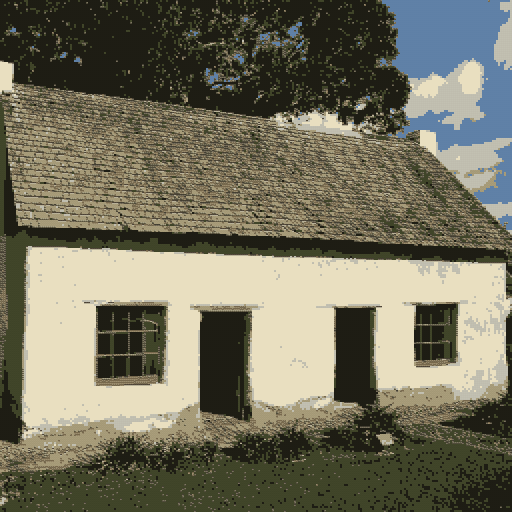
\includegraphics[width=\textwidth,width=90mm]{obrazy/house_R2_K12_P1_It10.png}
\caption{Rozmiar ramek: 2 liczba klastrów:12 powtórzenia: 1 iteracje: 10 }
\end{figure}

\begin{figure}[!htbp]
\centering
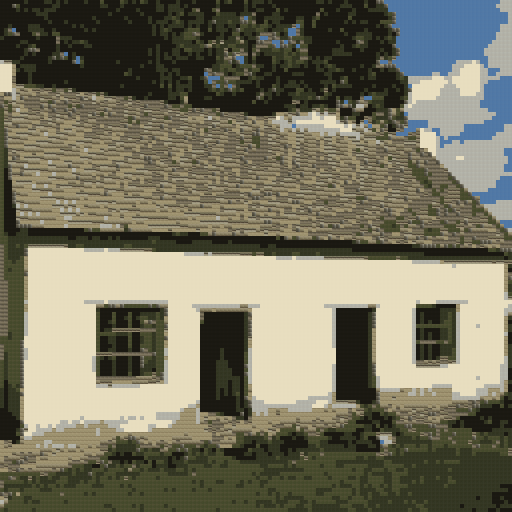
\includegraphics[width=\textwidth,width=90mm]{obrazy/house_R4_K12_P1_It10.png}
\caption{Rozmiar ramek: 4 liczba klastrów:12 powtórzenia: 1 iteracje: 10 }
\end{figure}

\begin{figure}[!htbp]
\centering
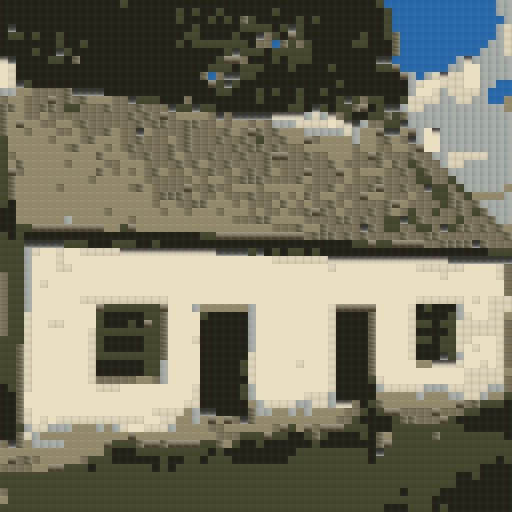
\includegraphics[width=\textwidth,width=90mm]{obrazy/house_R8_K12_P1_It10.png}
\caption{Rozmiar ramek: 8 liczba klastrów:12 powtórzenia: 1 iteracje: 10 }
\end{figure}

\begin{figure}[!htbp]
\centering
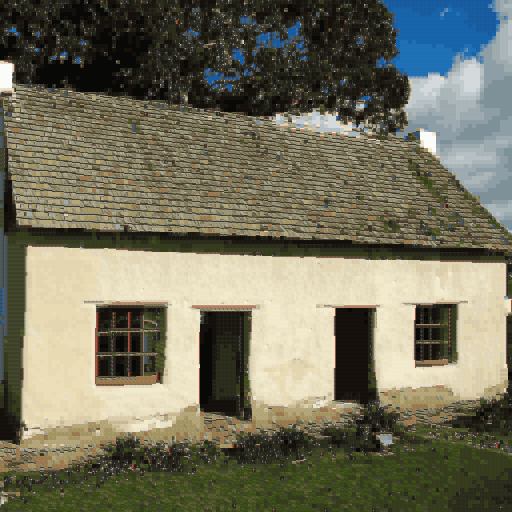
\includegraphics[width=\textwidth,width=90mm]{obrazy/house_R4_K128_P1_It10.png}
\caption{Rozmiar ramek:4 liczba klastrów:128 powtórzenia: 1 iteracje: 10 }
\end{figure}
\FloatBarrier
}

\subsubsection{duck.png}
{
Poniżej obrazy dla róznych rozmiarów ramek
\begin{figure}[!htbp]
\centering
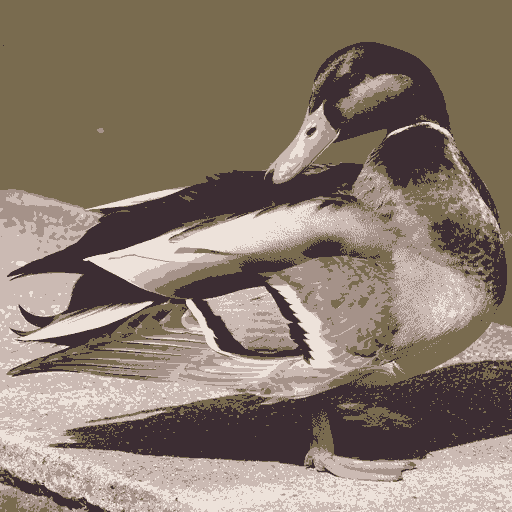
\includegraphics[width=\textwidth,width=90mm]{obrazy/duck_R1_K5_P1_It10.png}
\caption{Rozmiar ramek:1 liczba klastrów:5 powtórzenia: 1 iteracje: 10 }
\end{figure}

\begin{figure}[!htbp]
\centering
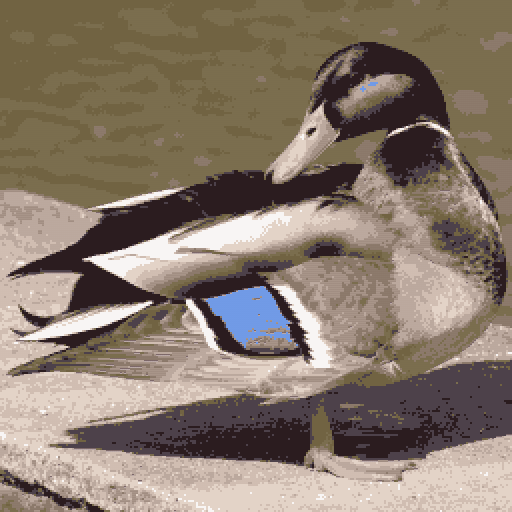
\includegraphics[width=\textwidth,width=90mm]{obrazy/duck_R2_K12_P1_It10.png}
\caption{Rozmiar ramek:2 liczba klastrów:12 powtórzenia: 1 iteracje: 10 }
\end{figure}

\begin{figure}[!htbp]
\centering
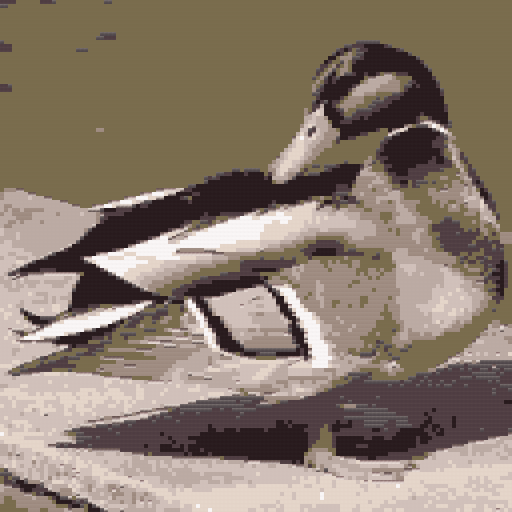
\includegraphics[width=\textwidth,width=90mm]{obrazy/duck_R4_K12_P1_It10.png}
\caption{Rozmiar ramek:4 liczba klastrów:12 powtórzenia: 1 iteracje: 10 }
\end{figure}

\begin{figure}[!htbp]
\centering
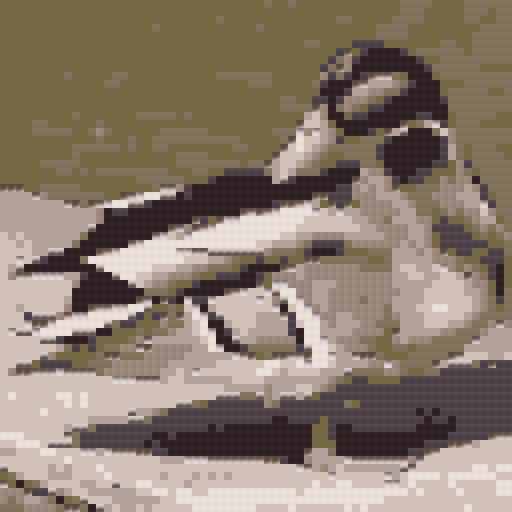
\includegraphics[width=\textwidth,width=90mm]{obrazy/duck_R8_K12_P1_It10.png}
\caption{Rozmiar ramek:8 liczba klastrów:12 powtórzenia: 1 iteracje: 10 }
\end{figure}

\begin{figure}[!htbp]
\centering
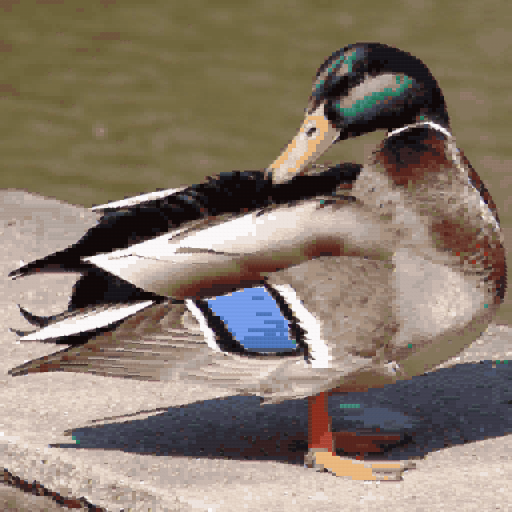
\includegraphics[width=\textwidth,width=90mm]{obrazy/duck_R4_K128_P1_It10.png}
\caption{Rozmiar ramek:4 liczba klastrów:128 powtórzenia: 1 iteracje: 10 }
\end{figure}
\FloatBarrier
}

\subsubsection{iris.png}
{

Poniżej obrazy dla róznych rozmiarów ramek
\begin{figure}[!htbp]
\centering
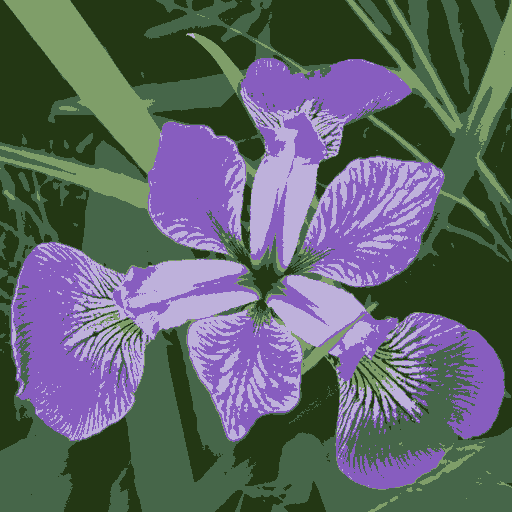
\includegraphics[width=\textwidth,width=90mm]{obrazy/iris_R1_K5_P1_It10.png}
\caption{Rozmiar ramek:1 liczba klastrów:5 powtórzenia: 1 iteracje: 10 }
\end{figure}

\begin{figure}[!htbp]
\centering
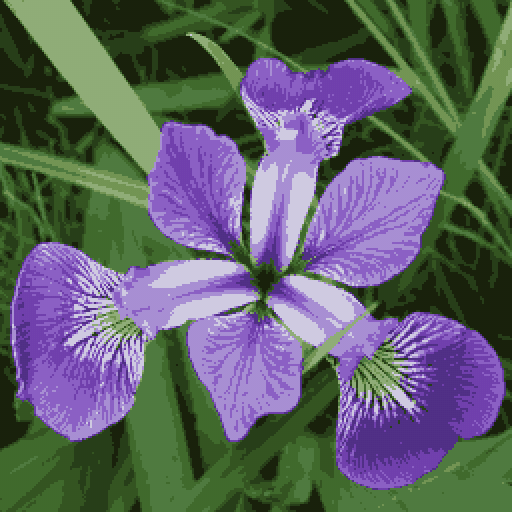
\includegraphics[width=\textwidth,width=90mm]{obrazy/iris_R2_K12_P1_It10.png}
\caption{Rozmiar ramek:2 liczba klastrów:12 powtórzenia: 1 iteracje: 10 }
\end{figure}

\begin{figure}[!htbp]
\centering
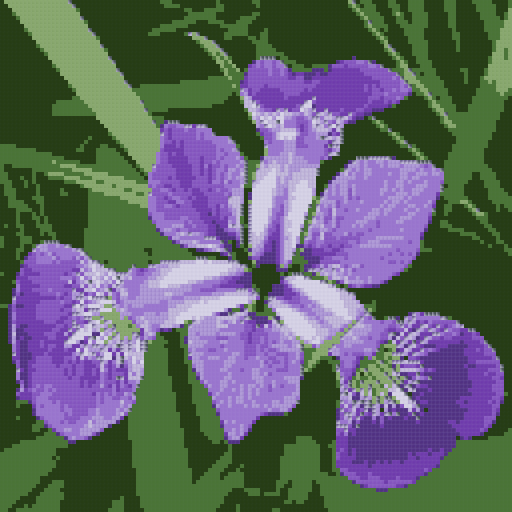
\includegraphics[width=\textwidth,width=90mm]{obrazy/iris_R4_K12_P1_It10.png}
\caption{Rozmiar ramek: liczba klastrów: powtórzenia: 1 iteracje: 10 }
\end{figure}

\begin{figure}[!htbp]
\centering
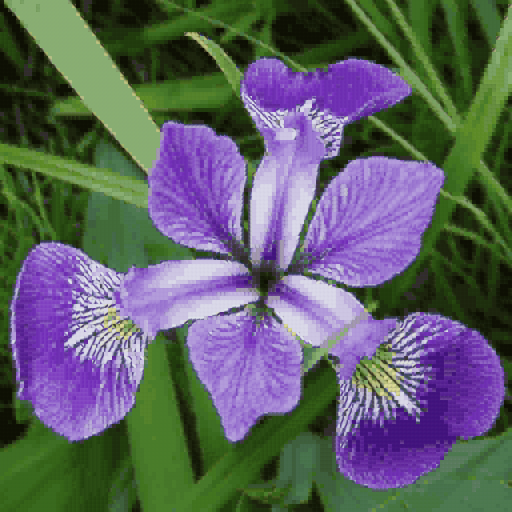
\includegraphics[width=\textwidth,width=90mm]{obrazy/iris_R4_K128_P1_It10.png}
\caption{Rozmiar ramek:4 liczba klastrów:128 powtórzenia: 1 iteracje: 10 }
\end{figure}

\begin{figure}[!htbp]
\centering
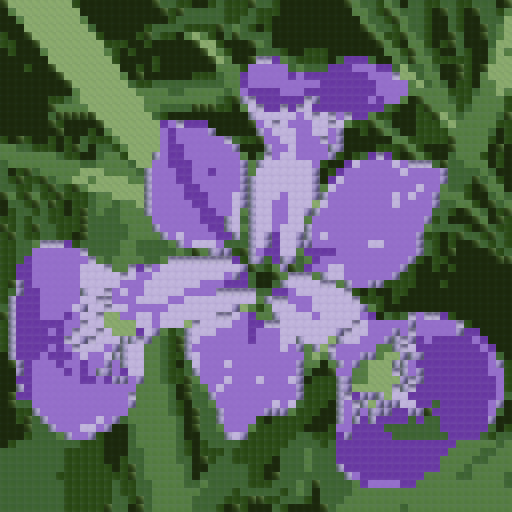
\includegraphics[width=\textwidth,width=90mm]{obrazy/iris_R8_K12_P1_It10.png}
\caption{Rozmiar ramek:8 liczba klastrów:12 powtórzenia: 1 iteracje: 10 }
\end{figure}
\FloatBarrier
}

\subsubsection{lenna.png}
{
Poniżej obrazy dla róznych rozmiarów ramek
\begin{figure}[!htbp]
\centering
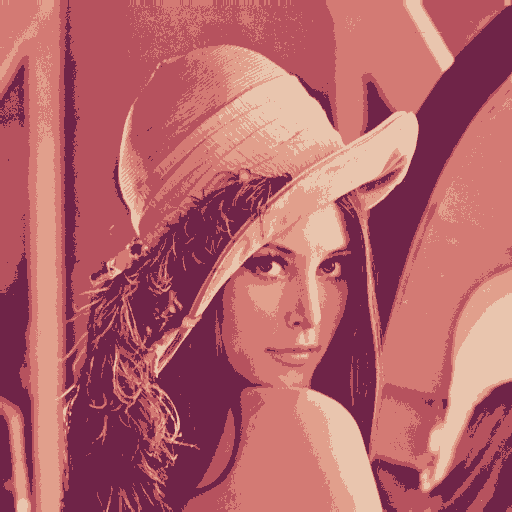
\includegraphics[width=\textwidth,width=90mm]{obrazy/lenna_R1_K5_P1_It10.png}
\caption{Rozmiar ramek:1 liczba klastrów:5 powtórzenia: 1 iteracje: 10 }
\end{figure}

\begin{figure}[!htbp]
\centering
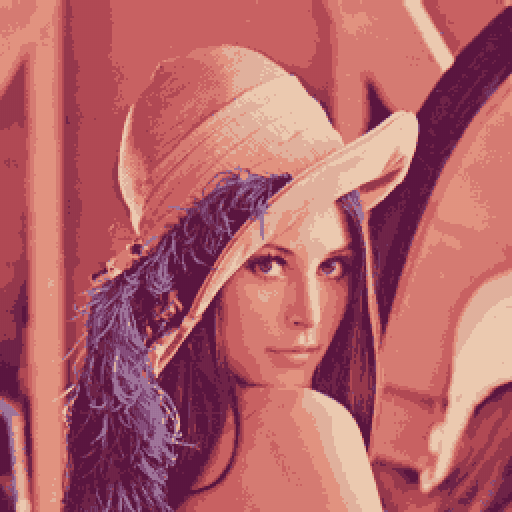
\includegraphics[width=\textwidth,width=90mm]{obrazy/lenna_R2_K12_P1_It10.png}
\caption{Rozmiar ramek:2 liczba klastrów:12 powtórzenia: 1 iteracje: 10 }
\end{figure}

\begin{figure}[!htbp]
\centering
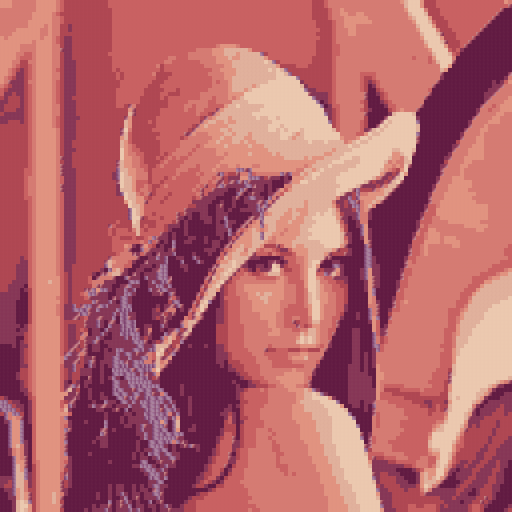
\includegraphics[width=\textwidth,width=90mm]{obrazy/lenna_R4_K12_P1_It10.png}
\caption{Rozmiar ramek:4 liczba klastrów:12 powtórzenia: 1 iteracje: 10 }
\end{figure}

\begin{figure}[!htbp]
\centering

\includegraphics[width=\textwidth,width=90mm]{obrazy/lenna_R8_K128_P1_It10.png}
\caption{Rozmiar ramek:8 liczba klastrów:128 powtórzenia: 1 iteracje: 10 }
\end{figure}

\begin{figure}[!htbp]
\centering
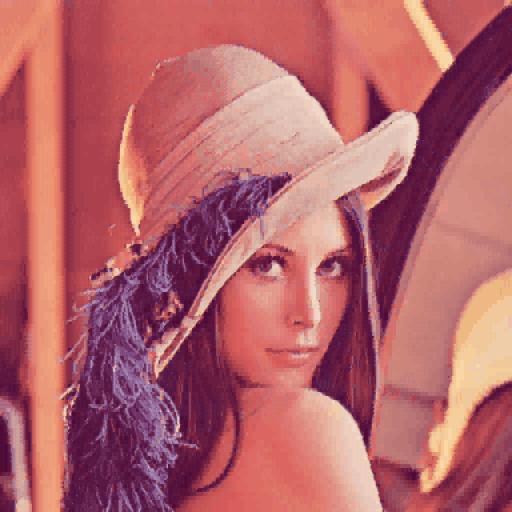
\includegraphics[width=\textwidth,width=90mm]{obrazy/lenna_R4_K256_P1_It10.png}
\caption{Rozmiar ramek:4 liczba klastrów:256 powtórzenia: 1 iteracje: 10 }
\end{figure}
\FloatBarrier
}

}

}

\section{Dyskusja}
{
Na podstawie uzyskanych wyników stwierdzamy, że metoda k-średnich na zbiorze irysów wykazuje się porównywalną
skutecznością na poziomie około 80\% bez względu czy została użyta opcja normalizacji czy też standaryzacji.
Jest to spowodowane tym, że dane na wejściu były już wcześniej dobrze ułożone, mamy tu na myśli zarówno podobny
zakres wartości jak i te same jednostki. Metoda k-średnich na zbiorze win odznacza się wielką różnicą w przypadku
skorzystania z opcji normalizacji lub standaryzacji. W przypadku jej użycia skuteczność klasteryzacji znacząco się
zwiększa. Jest to spowodowane tym, że zbiór win nie został wcześniej uporządkowany i występuje wiele wymiarów z
różnymi zakresami oraz jednostkami. Ma to taką konsekwencje, że część wymiarów wpływa silniej niż inne na wyniki
klasteryzacji. Metoda k-średnich dla zbioru abalone najlepiej opisują załączone grafiki - korzystanie z opcji
normalizacji lub standaryzacji ma ogromny wpływ na jakość wyników, informacja o skuteczności nie jest w tym przypadku
miarodajna w porównaniu zawartości kolumny płeć. Algorytm Kohonena dla danych abalone ma podobną cechę jak metoda
k-średnich dla tego samego zbioru danych czyli skuteczność około 50\%. Przez to nie jest możliwe dobre przewidzenie
rozkładu płci. Pomimo całego geniusza tych metod nie zawsze są one do końca skuteczne i warto wykonać analizę
otrzymanych wyników. Podobnie jak w metodzie k-średnich dla zbioru irysów normalizacja lub standaryzacja znacząco
nie wpływa na uzyskaną jakość klasteryzacji. Metoda Kohonena odznaczyła się znacznie wyższą skutecznością przy
skorzystaniu z standaryzacji natomiast wykonywanie normalizacji nie miało zbyt dużego sensu gdyż wyniki były bardzo
porównywalne z tymi uzyskanymi na danych wejściowych bez żadnej ingerencji.

}

\section{Wnioski}
{
Podsumowując wykonane zadanie wnioskujemy, że:
\begin{itemize}
\item Przy danych, których poszczególne wymiary mają różny zakres wartości lub jednostki wcześniejsze zastosowanie
normalizacji lub standaryzacji wpływa poprawę jakości klasteryzacji. W przypadku gdzie wymiary są w miarę jednolite
pod względem zakresu normalizacja nie wpływa znaczącą na wynik klasteryzacji
\item Z naszych obserwacji wynika, że metoda k-średnich jest w stanie wykonać lepszą klasteryzacje niż algorytm
Kohonena przy tej samej liczbie iteracji.
\item Dla zbiorów irysów i win uzyskana klasteryzacja pokrywa się w znaczącym stopniu z oczekiwaną
(z klasami podanymi w zbiorach danych)
\end{itemize}
}

\begin{thebibliography}{0}
\bibitem{l2short}\url{ http://wikizmsi.zut.edu.pl/uploads/6/6f/InstrukcjaGaz.pdf}
\bibitem{l2short} \url{https://en.wikipedia.org/wiki/K-means\_clustering}
\bibitem{l2short} \url{http://www.michalbereta.pl/dydaktyka/WdoSI/lab_neuronowe_II}
\end{thebibliography}

{

}

\end{document}
